\documentclass[a4paper,twoside,adobefonts]{ctexbook}
\usepackage[xetex,hidelinks,bookmarks]{hyperref}
\usepackage{ltxtable}
\usepackage{pdfpages}
\usepackage{thesis}
\usepackage{verbatim}
\begin{document}

%前面几页不需要页眉页脚
\pagestyle{empty}

%封面
%    \begin{titlepage}
	\begin{center}
		\noindent\includegraphics[height=2.5cm]{figures/bupt_handwriting.eps}\\
		\vspace{4mm}	%本身有6.3mm的间隔
		\heiti\zihao{1}\textbf{本~科~毕~业~设~计~(论文)} \\
		\vspace{8mm}
		\noindent\includegraphics[height=3.2cm]{figures/bupt_logo.eps}\\
		\vspace{8mm}
		\setlength{\arrayrulewidth}{1pt}
		\begin{tabular}{@{}p{54.2pt}@{}p{233.4pt}}
      \heiti\zihao{3}\textbf{题目:} & \heiti\zihao{3}\hfill 基于MVVM架构的         \hfill \mbox{~} \\[-4pt] \cline{2-2}
			\heiti\zihao{3}\mbox{~}	      & \heiti\zihao{3}\hfill 课程管理系统设计与实现 \hfill \mbox{~} \\[-4pt] \cline{2-2}
		\end{tabular}\\
		\vspace{4mm}
    \begin{tabular}{@{}p{70pt}@{}p{180pt}@{}}
      \songti\zihao{3}\textbf{姓\qquad 名} & \songti\zihao{3}\hfill 陈杰      \hfill \mbox{~}\\[-4pt] \cline{2-2} %姓名
			\songti\zihao{3}\textbf{学\qquad 院} & \songti\zihao{3}\hfill 软件学院  \hfill \mbox{~}\\[-4pt] \cline{2-2}	%学院
			\songti\zihao{3}\textbf{专\qquad 业} & \songti\zihao{3}\hfill 软件工程  \hfill \mbox{~}\\[-4pt] \cline{2-2}	%专业
			\songti\zihao{3}\textbf{班\qquad 级} & \songti\zihao{3}\hfill 2010211501\hfill \mbox{~}\\[-4pt] \cline{2-2} %班级
			\songti\zihao{3}\textbf{学\qquad 号} & \songti\zihao{3}\hfill 10212043  \hfill \mbox{~}\\[-4pt] \cline{2-2}	%学号
			\songti\zihao{3}\textbf{班内序号}    & \songti\zihao{3}\hfill 11        \hfill \mbox{~}\\[-4pt] \cline{2-2}	%班内序号
			\songti\zihao{3}\textbf{指导教师}    & \songti\zihao{3}\hfill 刘禾      \hfill \mbox{~}\\[-4pt] \cline{2-2}	%指导教师
		\end{tabular}\\
		\vspace{12mm}
		\songti\zihao{3}\textbf{2014~年~6~月}
	\end{center}
\newpage
\rule{0pt}{0pt}
\newpage
    \end{titlepage}



%诚信声明
%\include{parts/statement}

%中文摘要
\newpage
\begin{center}
	\heiti\zihao{3}\textbf{基于 MVVM 架构的课程管理系统的设计与实现}
\end{center}
\begin{center}
	\heiti\zihao{-3}\textbf{摘\quad 要}
\end{center}
\vspace{2.5mm}
\songti\zihao{-4}

Model-View-ViewModel (MVVM) 模式是 Model-View-Controller (MVC) 模式的一种特例,2005 年由 Microsoft 提出并首次应用于 Windows Presentation Framework (WPF),MVVM 模式将 MVC 架构模式与 Observer 模式配合使用,在 Model、ViewModel 与 View 之间通过 DataBinding 建立关系,解决了图形用户界面(Graphical User Interface)开发中对异步事件处理的难点,近年来十分受到业界的重视。

本文以课程管理系统的设计与实现为例,对比分析 MVVM 模式的开发性能,同时尝试对 MVVM 模式在 JavaScript 语言平台上的实现提出改进方案。借助 JavaScript 语言平台支持函数式编程的特性,在 MVVM 框架中引入 Functional Reactive Programming (FRP) 的设计思想,并从 Reactive Programming 的角度分析讨论 MVVM 模式在处理异步逻辑方面的优越性、设计基于 Monad 对象实现 ViewModel 的改进框架。

\vspace{3mm}
\zihao{-4}\heiti\textbf{关键字}\quad \songti MVVM \quad 富应用 \quad Reactive Programming \quad 课程管理系统



%英文摘要
\begin{center}
\zihao{3}\textbf{An MVVM Based Course Management System}
\end{center}
\begin{center}
\zihao{-3}\textbf{ABSTRACT}
\end{center}
\vspace{2mm}
\zihao{-4}

Model-View-ViewModel (MVVM) design pattern is a pattern providing a resolution to asynchronous programming of Graphical User Interface (GUI) which is introduced into Windows Presentation Framework (WPF) at 2005 by Microsoft. Based on Observer Pattern, MVVM uses feature called DataBinding to make connection between Model, ViewModel and View objects. With it's success in handling asynchronous events, MVVM has been adopted widely Rich Interaction Applications (RIAs).

The subject of this article is to design a Course Management system based on MVVM framework, and, introduce improvement to MVVM development on JavaScript platform.

A typical Object-oriented MVVM implementation on JavaScript platform does not make use of functional programming ability of JavaScript. The article tries to introduce the idea of Functional Reactive Programming (FRP) into MVVM design and analyse the use of Observer in typical MVVM implementation from the view of Functional Programming Language. Then, bring up the ViewModel built by Monad objects.

\vspace{3mm}
\zihao{-4}{\bfseries KEY WORDS}\quad MVVM \quad FRP \quad Asynchronous Programming \quad Management System


\frontmatter{Roman} %开始罗马页数计数

\pagestyle{plain} %显示页脚(页码)

%目录
\tableofcontents

\mainmatter	%开始阿拉伯数字计页数

%从正文开始加入页眉和页脚
\pagestyle{fancy}

%正文
\chapter{概述}

本章介绍课程管理系统的项目背景并简要阐述 Model-View-ViewModel (MVVM) 模式、Functional Reactive Programming (FRP) 方法的核心思想及特性。

\section{项目背景}

用户交互(User Interaction)在消费级产品开发中的地位近年来正不断提升,交互设计和实现正成为产品开发中最重要也最复杂的环节之一。随着互联网的发展、富交互应用(Rich Interaction Application, RIA)的兴起,交互设计正走向越来越复杂的方向。使用传统的命令式编程(Imperative Programming)实现用户交互逻辑的局限性也不断显现出来。

Microsoft 在 Windows Presentation Framework (WPF) 中引入的 Model-View-ViewModel(MVVM) 模式近年来得到了相当广泛的关注和应用~\footnote{Wikipedia: Model View ViewModel}。MVVM模式作为如今最成功的图形用户界面(Graphical User Interface, GUI)开发模式之一,将声明式方法引入用户交互开发,解决了命令式编程方法在处理异步逻辑时难于维持代码逻辑连续性的问题。

课程管理系统作为面向业务产品的典型代表,工程规模足够体现设计模式的各项性能。本文以课程管理产品的设计与开发为例,尝试解释 MVVM 设计模式的设计方法,并从 FRP 的角度解释 MVVM 模式中 ViewModel 部分的设计,在此基础上使用 monad 结构~\cite{raey}开发 MVVM 框架并测试该框架在课程管理系统中实际进行富交互应用开发的性能。

\section{Model-View-ViewModel~模式}

经典的 MVC 模式~\footnote{Wikipedia: Model–view–controller} 将系统分成 Model(模型)、View(视图)、Controller(控制器) 三个部分: Model 对象用于处理数据和业务操作、View 对象控制视图逻辑、Controller 负责处理用户操作。MVC 架构作为许多互联网产品和应用的基础架构在各大开发平台都有成熟的解决方案和技术框架~\footnote{如 Ruby-on-Rails、ThinkMVC 等广泛应用的 Web 框架都基于 MVC 架构进行开发}。

\begin{figure}[!h]
\begin{center}
\includegraphics[scale=0.5]{figures/pattern-mvc.pdf}
\caption{MVC 模式\label{MVCOverview}}
\end{center}
\end{figure}

Microsoft 作为用户交互领域的先驱,最早在 2005 年由工程师 Martin Fowler 提出了 MVVM 架构并应用于 Windows Presentation Framework。

\begin{figure}[!h]
\begin{center}
\includegraphics[scale=0.7]{figures/pattern-mvvm.pdf}
\caption{MVVM 模式\label{MVVMOverview}}
\end{center}
\end{figure}

Model-View-ViewModel (MVVM) 模式是 Model-View-Controller (MVC) 模式的一种特例(见图~\ref{MVVMOverview}): MVC 模式中 Controller 负责进行的界面业务逻辑部分抽象为 ViewModel 以及 Binder 组合。一方面利用 ViewModel 管理交互状态、另一方面通过 Binder 将状态通过 View 进行展示。用户产生的交互事件也经由 Binder 传递至 ViewModel 对用户界面的状态以及 Model 状态产生影响。

MVVM 模式的一大设计亮点在于“ViewModel 继承于 Model” 即: ViewModel 可以将另一个 ViewModel 实例作为 Model 进行数据请求。这是 ViewModel 与 Controller 之间最大的不同,也是 ViewModel 较 Controller 实现拥有更高的可复用性以及更良好的可测试性的原因。

另外,MVVM 模式解除了 Controller 代码与视图实现之间的耦合关系,界面设计人员仅需要在XAML(对WPF的情况)文档中描述视图对象所需要绑定(bind)的数据位置(属性名称)即可完成用户交互设计任务,而在 MVC 模式中设计者需要书写 Controller 代码以描述视图对象所需要的呈现数据。

MVVM 模式在普遍用于用户交互开发的 JavaScript 语言中也得到了类似的实现,如 AngularJS、KnockoutJS 等开发框架。

\section{Functional Reactive Programming (FRP)}

Functional Reactive Programming (FRP) 是使用声明式 (Declarative) 方法描述系统行为的编程方法。FRP 的主要思想是将系统抽象为 $行为(Behaviors)$ 和 $事件(Events)$,使用行为表示系统中随时域连续变化的值、事件表示一系列按一定时序触发的离散值~\cite{Wan:2000:FRP:358438.349331}。最初,FRP 方法被应用于 Haskell 的 Functional Reactive Animation (Fran) 的核心实现~\cite{Elliott:1997:FRA:258949.258973}。后来,FRP 方法被广泛的用于计算机视觉、机器人以及其他控制系统的设计和实现。

简而言之,FRP 抽象系统为用户与函数(Behavior)的交互,用户事件作为函数的自变量,而模型/用户视图作为函数作用的因变量。

随着 FRP 理论的成熟与富交互应用的发展,FRP 的影响也逐渐延伸到应用开发的前沿领域,出现了许多成熟的 FRP 开发框架,如 Objective C 平台下的 ReactiveCocoa,.NET Framework 下的 ReactiveUI 以及 JavaScript 平台下的 Reactive.js 等~\footnote{虽然这些框架是实现在命令式语言平台的 Reactive Programming 框架,这里还是沿用 Haskell 中 FRP 的名称}。

FRP 方法与 MVVM 使用的 Observer 模式具有很高的相似性,本文将在后面的章节围绕此问题进行一番讨论并提出作者对 MVVM 架构模式的理解。

后文分成五个部分: 第二章、第三章分别介绍系统的需求分析和概要设计,第四章引入有关MVVM模式与 Reactive Programming 的讨论、描述 ReactiveVM 的设计思路,第五章讨论实现过程中出现的探索性过程,第六章对项目的开发过程进行一个总结并描述一下对未来研究方向的展望。


\chapter{需求分析}

本章主要对课程管理系统的需求进行分析,通过建立目标模型、用户用例模型、系统领域模型对系统的功能性需求以及非功能性需求进行准确的确定,明确系统的开发边界。

\section{目标模型}

目标模型是需求工程用于推导各级需求的关键模型,从任意一项目标出发向上推导更抽象、更概括的目标,向下推导更具体、更细致的需求。

\begin{figure}[!h]
  \begin{center}
    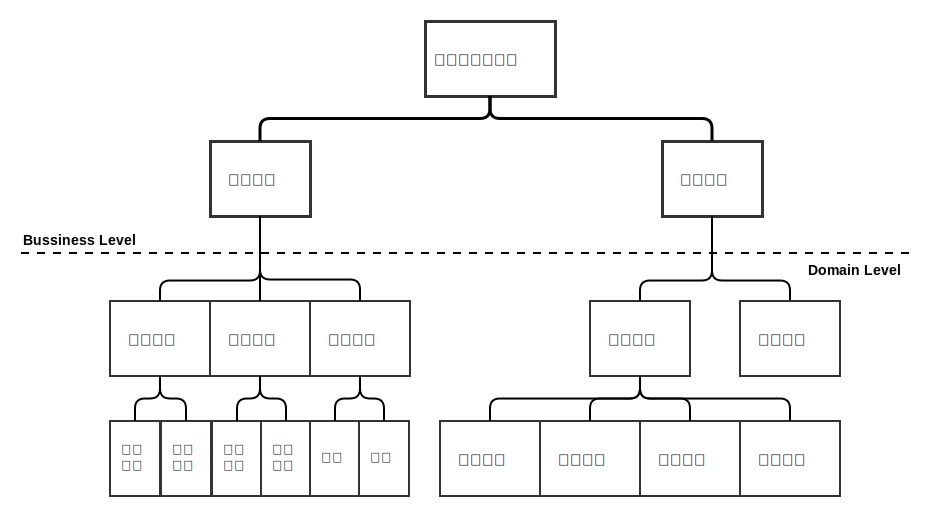
\includegraphics[width=\textwidth]{figures/goal.pdf}
    \caption{课程管理系统目标模型(Goal Model)示意图\label{GoalModel}}
  \end{center}
\end{figure}

图~\ref{GoalModel} 列出了系统业务目标和领域目标(需求)之间的层次关系。图中虚线所标识的位置是业务目标(Bussiness Goal)与领域目标的分界线,业务目标指的是在现实中实现这些业务所需要了解的目标; 领域目标指的是进行领域设计时需要了解的目标。将目标模型继续向下推导我们可以达到产品目标。

目标模型通过站在关系人(Stakeholder)的角度确定系统边界,系统目标可以通过对应关系直接转换为产品需求(\nameref{sec:appendix-requirement-table})

\section{用例模型}

在需求获取的过程中使用用例模型能够更清晰的与对方展开需求沟通。

\begin{figure}[!h]
  \begin{center}
    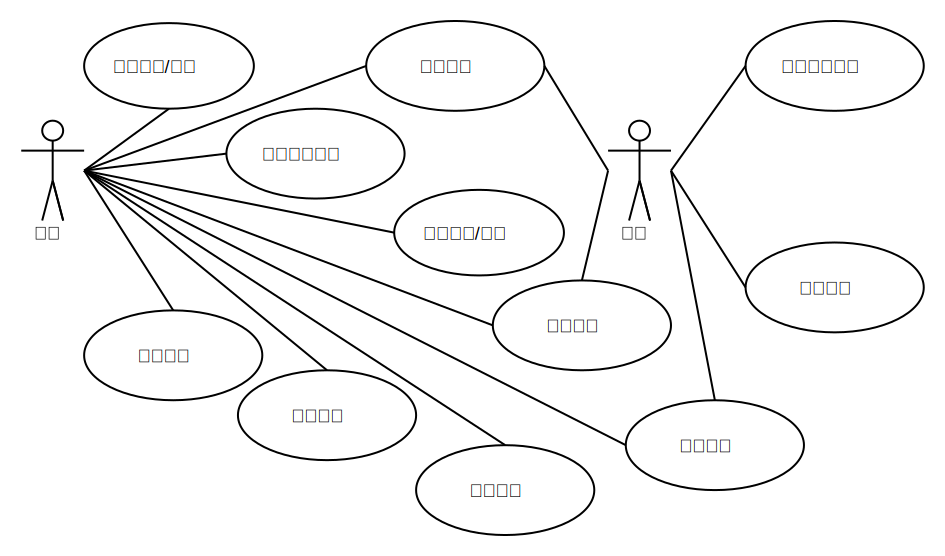
\includegraphics[width=\textwidth]{figures/uc.pdf}
    \caption{目标系统用户用例(Use Case)示意图\label{UseCase}}
  \end{center}
\end{figure}

图~\ref{UseCase} 所示的用户用例涉及多个交互,比较复杂,下文使用文本对不同的交互进行描述。可以看出课程管理系统的业务是导师与学员两类主要用户角色所主导的。

时间顺序上,每个课程拥有独立的过程控制点(阶段),系统根据课程所处的不同阶段对能对课程应用的业务操作进行控制和管理。

\subsection {交互: 发布课程}

用户使用导师身份进入系统后,执行下面的操作:

\begin{enumerate}
  \item 进入“发布课程”模块
  \item 填写课程标题、课程描述、授课规模以及其他自定义课程信息
  \item 提交课程信息
\end{enumerate}

课程信息提交后课程条目会出现在课程列表中,选择条目可以查看到导师填写的课程详细信息。

\subsection {交互: 选择课程与课程录取}

用户使用学员身份进入系统后,与系统进行下面的交互:

\begin{enumerate}
  \item 进入“课程申请”模块
  \item 选择课程列表中的课程条目
  \item 查看课程详细信息
  \item 提交课程申请
\end{enumerate}

提交课程申请之后还可以进行下面操作:

\begin{itemize}
  \item 撤销课程申请: 撤销已提交但未通过的课程申请
\end{itemize}

用户使用导师身份进入系统后,与系统进行下面的交互:

\begin{enumerate}
  \item 选择课程列表中的课程条目
  \item 进入课程详细信息
  \item 选择/取消课程申请列表中的学员条目
\end{enumerate}

还可以进行下面操作:

\begin{itemize}
  \item 录取结束: 完成所有录取操作(未来将不可增加/删除学员)
\end{itemize}

完成录取后,对应的课程就进入可以进行任务发布的状态。

\subsection {交互: 发布任务与完成任务}

用户使用导师身份进入系统后,与系统进行下面的交互:

\begin{enumerate}
  \item 选择课程列表中的课程条目
  \item 进入课程详细信息
  \item 选择“新任务”
  \item 输入任务所需的基本信息(标题、要求、截止时间)
  \item 提交任务信息
\end{enumerate}

用户使用学员身份进入系统后,与系统进行下面的交互:

\begin{enumerate}
  \item 选择课程列表中的课程条目
  \item 进入课程详细信息
  \item 选择未完成的任务条目
  \item 填写任务需要完成的项目(以在线表格或者文件上传等形式)
  \item 提交答案以完成任务~\footnote{图~\ref{UseCase} 中的“完成任务”即学员进行答案提交的行为}
\end{enumerate}

完成任务后学员可继续提交、更新任务的答案直到导师做出任务评价。

\subsection {交互: 评价/评分}

用户使用导师身份进入系统后,与系统进行下面的交互:

\begin{enumerate}
  \item 选择课程列表中的课程条目
  \item 进入课程详细信息
  \item 进入课程学员列表
  \item 选择课程中的一位学员、查看任务列表
  \item 查看/下载学员提交的任务内容
  \item 填写任务评价/评分
  \item 提交评分表格
\end{enumerate}

在课程结束前,导师还会与系统进行下面的交互:

\begin{enumerate}
  \item 选择课程列表中的课程条目
  \item 进入课程详细信息
  \item 进入课程学员列表
  \item 选择课程中的一位学员、查看任务列表
  \item 填写该学员的课程评价/评分
  \item 提交评分表格
\end{enumerate}

导师完成课程评分后可在学员列表直接查看到学员的课程得分。 学员可在任务列表查看到导师发布的任务评价,在课程的详细信息页面查看到导师发布的课程评分。

\section{系统领域模型}

建立系统领域模型可以帮助理解系统运行的外部环境以及系统开发的边界位置。

\begin{figure}[!h]
  \begin{center}
    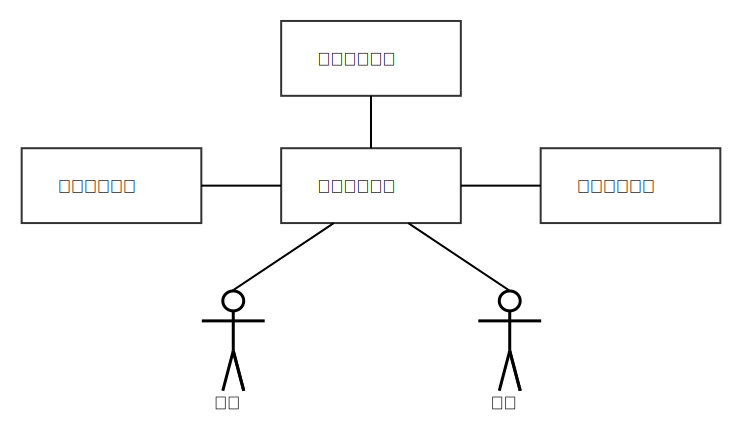
\includegraphics[scale=0.6]{figures/domain.pdf}
    \caption{目标领域模型(Domain Model)示意图\label{DomainModel}}
  \end{center}
\end{figure}

图~\ref{DomainModel} 所示为系统的领域模型示意图,图中的系统分别负责:

\begin{itemize}
  \item 开放身份系统(Open Identity System),负责用户身份的验证,以便用户能在不同系统中使用同一个身份
  \item 邮件服务系统,用于处理业务邮件请求(如发送通知、提醒)
  \item 归档管理系统,管理来自不同系统的归档,提供归档和归档的索引及下载服务
  \item 课程管理系统,本项目的目标系统,处理课程管理方面的业务请求
\end{itemize}

领域模型能够帮助明确系统边界以及与系统相关的服务接口,在验证需求有效性时能起到指导性作用。

作为面向业务产品领域的关键知识,项目对课程管理系统的业务过程建立了业务过程模型(Business Process Model, BPM),使用图形化的语言简单清晰地描述了系统所需要完成的业务逻辑。

\begin{figure}[!h]
  \begin{center}
    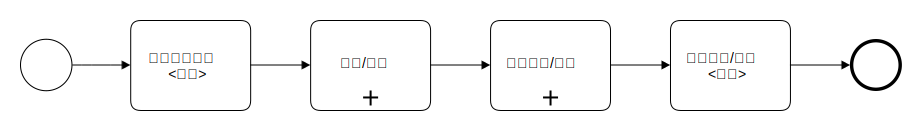
\includegraphics[width=\textwidth]{figures/bpm.pdf}
    \caption{业务过程模型示意图(概览)\label{BPMOverview}}
  \end{center}
\end{figure}

图~\ref{BPMOverview} 展示了系统最上层业务逻辑的结构由课程信息的发布、学员的匹配(申报/录取)、课程过程控制(任务发布/完成)、归档整理四个主要业务版块构成,更详细的业务过程模型可参考~\nameref{sec:appendix-bpm}。

\section{小结}

在构造需求模型的过程中,维持需求的有效性、一致性、完备性、真实性和可检验性是有一定难度的,在本项目的需求模型构造环节中需求的发现、验证和整理按照图~\ref{RequirementExtraction} 所展示的过程进行,通过维持需求-目标的可追溯性来达到上述需求质量要求。

\begin{figure}[!h]
  \begin{center}
    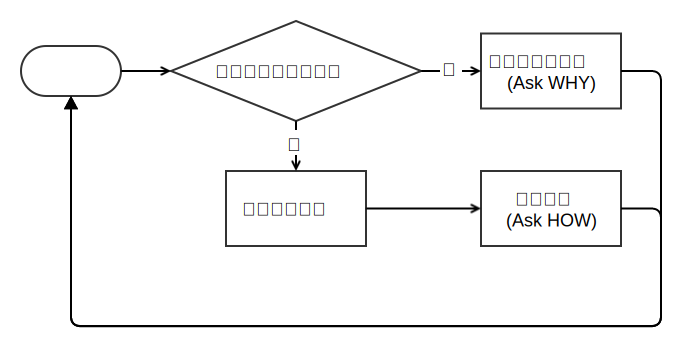
\includegraphics[scale=0.6]{figures/process-requirement.pdf}
    \caption{构造可追溯的需求发现-验证流程\label{RequirementExtraction}}
  \end{center}
\end{figure}

在与系统客户讨论和确定需求的过程中,业务过程模型发挥着很大的作用,通过与系统客户在系统业务上达成共识能够很快的发现与业务相关的功能性需求。

需求分析是软件项目开发中非常重要的环节,需求分析的过程中所产生需求文档在沟通过程中能够发挥巨大的作用。在文档中恰当的使用各类图形化的表达方法也有助于对系统中重要需求的理解与发现。

下一章将叙述从产品需求出发进行系统概要设计的过程,与需求的构造模式相似,概要设计内部以及概要设计与需求之间保持着可追溯的关系。


\chapter{概要设计}

本节描述系统的概要设计过程以及系统概要设计。课程管理系统的设计与办公自动化(Office Automation, OA)系统同为面向业务的应用拥有很多相似的设计,本项目在设计上也参考了典型的 OA 系统设计模式,同时借鉴 RIA 系统的设计思想,使项目既能保持业务的高度一致性,又能应对开发过程中所发生的各类变更。

\section{体系结构设计}

图~\ref{Architecture} 简单描述了系统的基础架构。

\begin{figure}[!h]
  \begin{center}
    \includegraphics[scale=0.7]{figures/architecture.pdf}
    \caption{系统架构示意图\label{Architecture}}
  \end{center}
\end{figure}

基于经典的 Client/Server (C/S) 架构模式。在 C/S 模式的基础上,基于浏览器这一特殊的执行环境(Execution Context),客户端程序并不直接部署在用户终端上,架构中加入了内容分发网络用于分发静态的客户端程序数据。

接下来,与现在典型的 MVVM 应用方式不同\footnote{Angular.js、Knockout.js等流行的JavaScript实现将MVVM作为客户端框架进行实现},我们在C/S的基础架构上,应用MVVM架构(图~\ref{ArchitectureMVVM})

\begin{figure}[!h]
  \begin{center}
    \includegraphics[scale=0.7]{figures/architecture-mvvm.pdf}
    \caption{MVVM 系统架构示意图\label{ArchitectureMVVM}}
  \end{center}
\end{figure}

服务器提供MVVM框架中模型(Model)的支持,负责响应业务请求和维护业务数据,客户端提供视图(View)以及视图模型(ViewModel)负责业务数据的呈现逻辑和用户事件的处理\footnote{服务器与客户端之间的通信属于ViewModel的一部分}。

下面将分两个小节分别介绍服务器和客户端的二级架构方案。

\subsection{服务器架构方案}

将服务器部分作为Model进行设计的一大特点是服务器设计的轻量化,这与常见的RIA应用中的服务器设计是基本相符的,服务器为业务数据共享、权限管理等基本需求提供了支持。

\begin{figure}[!h]
  \begin{center}
    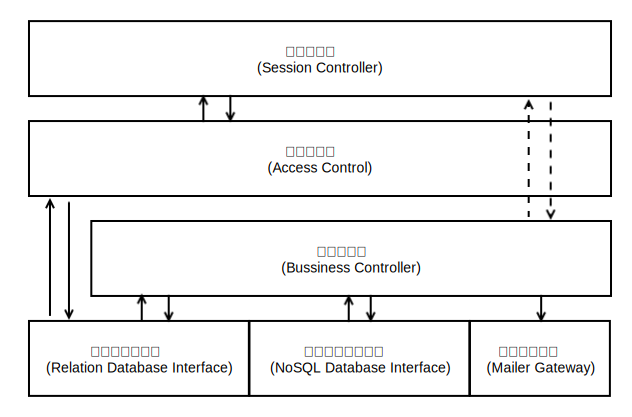
\includegraphics[scale=0.7]{figures/architecture-server.pdf}
    \caption{服务器架构示意图\label{ArchitectureServer}}
  \end{center}
\end{figure}

图~\ref{ArchitectureServer} 说明服务器的分层架构模式:

\begin{itemize}
  \item 顶层通过 HTTP/HTTPS 提供的会话层对会话状态进行管理
  \item 权限控制器提供账户服务
  \begin{itemize}
    \item 处理账户登录、注册等账户相关数据业务
    \item 拒绝超出权限范围的访问请求、保障用户逻辑输入的正确性
    \item 向业务逻辑层提供透明的用户认证机制
  \end{itemize}
  \item 业务逻辑层实现产生商业价值的业务逻辑
  \item 最下层为数据持久化以及外部服务层
\end{itemize}

服务器利用混合数据库模式,关系型数据库管理业务数据等强关系关联的数据、非关系型数据库处理会话数据等弱关系数据。(见~\ref{sec:Database})

\subsection{客户端架构方案}

上文中提到客户端实现整体架构中的View以及ViewModel部分

\begin{figure}[!h]
  \begin{center}
    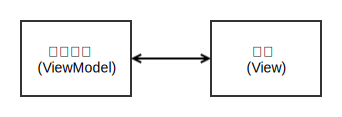
\includegraphics[scale=0.7]{figures/architecture-client.pdf}
    \caption{客户端架构示意图\label{ArchitectureClient}}
  \end{center}
\end{figure}

视图 (View) 在系统中被定义为一系列模板的集合,ViewModel 处理页面逻辑,经典 MVVM 模式当中的 DataBinding 模式由特殊的 ViewModel 实现。

\section{数据库设计\label{sec:Database}}

本项目主要使用关系型数据库系统(Relational Database System, RDBS)进行业务数据的管理。

在面向业务的系统构建,特别是 MVVM 模式构建的系统当中,对数据的清晰定义将影响到系统业务的稳定性、可靠性、可扩展性等多个重要的性能。定义良好的数据规格可以直接成为 MVVM 模式中 Model 定义的来源。

本节首先描述课程管理系统数据库的设计概要以及一些需要特别说明的设计概念,后面几个小节描述课程数据、表单数据、用户数据模型的设计方案。

\newpage

\subsection{数据库设计概要}

下图简单的列出了数据库设计(详见~\nameref{sec:appendix-database-diagram})

\begin{figure}[!h]
  \begin{center}
    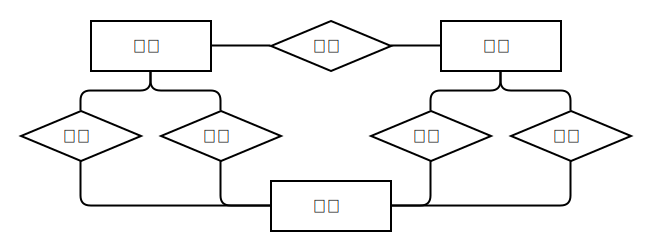
\includegraphics[scale=0.7]{figures/er.pdf}
    \caption{数据库E-R关系示意图\label{DatabaseOverview}}
  \end{center}
\end{figure}

系统主要有下面三类业务数据实体:

\begin{itemize}
  \item 课程数据实体
  \item 表单数据实体
  \item 用户数据实体
\end{itemize}

需要特别说明的是 \textbf{表单数据实体} 用于存储系统内其他实体所引用的表单定义。在现实的业务交往过程当中,业务的完成流程往往是基于表格的,创建业务管理系统的核心就在于对表单的创建、维护以及对填写好的表单进行归档、整理。因此,在系统的设计过程中通过创建通用的表单数据实体,将业务数据需求通过表单数据实体进行描述,能避免系统内对业务数据的检索,提高数据库的可扩展性以及系统的业务灵活度。

同时,系统内存在下面业务关系:

\begin{itemize}
  \item 选课业务关联
  \item 表单引用关联
  \item 标签/域关联~\footnote{为了让图形语言表达更清晰,本关联未在图~\ref{DatabaseOverview} 中得到体现。}
  \item 创建者关联
\end{itemize}

\textbf{标签/域关联} 是为了满足系统对系统内数据实体访问权限的细化控制需求而设定的配置数据,这是一组在所有实体上都可以实现的“接口”,实体通过限定“域(Scope)”确定有权限访问该实体的“标签(Tag)”。标签是对“搜索”逻辑的简化和抽象,使用标签机制可以更高效地完成对数据实体的筛选操作,基于标签的检索也能够更有效的保证数据库系统的安全性与可靠性。

\newpage

\subsection{课程实体设计}

课程实体由导师创建,用于存放课程业务数据,与表单数据之间有紧密的业务联系。

\begin{figure}[!h]
  \begin{center}
    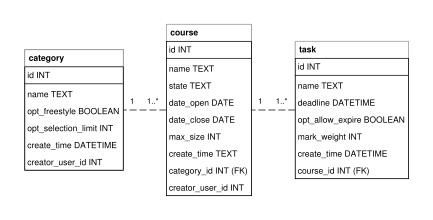
\includegraphics[width=\textwidth]{figures/eer-course.pdf}
    \caption{课程实体\label{DatabaseEntityCourse}}
  \end{center}
\end{figure}

\textbf{课程(course)} 是与课程管理系统的核心实体,包含了课程的基本信息。

\textbf{任务(task)} 为导师规划课程进展、检测教学成果提供了条件:

\begin{itemize}
  \item 系统可以借助评分权重和每一项任务的评分辅助导师给出学员的课程成绩。

  \item 任务表单由导师维护,添加任务时选取,学生应在截止时间内填写完成表单(作业)并提交,供导师查阅后给出评分。

  \item 任务截止之前(允许超时提交的情况下也包括截止之后)学员可多次提交更新。
\end{itemize}

\textbf{课类(category)} 的设计是为了解决更复杂的选课管理需求:

\begin{itemize}
  \item 课类为每门课程提供一份模板,课类下属的课程需“继承”自该课类(课程类目)
  \item 可由导师定义课类内的选课方案~\footnote{比如,“2010级企业实习实训”课类下,定义每名学员只能选取单一课程,在此课类下创建相关的实习实训职位,自主实习的学生可向负责导师申请添加新的职位信息,导师批准后即给与选取。}
  \item 开放学员选题的课类可由学员向指定导师提交课题,课题信息经过导师审核,经指定导师同意后加入课类
\end{itemize}

\newpage

\subsection{用户/账户实体设计}

用户账户实体存储了用户信息、用户权限等信息,应用层权限控制提供了存储条件。

\begin{figure}[!h]
  \begin{center}
    \includegraphics[width=\textwidth]{figures/eer-user.pdf}
    \caption{用户/账户实体\label{DatabaseEntityUser}}
  \end{center}
\end{figure}

用户在系统内的活动以~\textbf{用户(User)} 实体作为身份标识,\textbf{账户(Account)} 为需要连接的外部身份提供存储支持(如 OpenID 服务)。

数据库配置了基于用户-组-权限的数据结构以存储权限配置,有关权限控制的更多细节请参考~\ref{sec:ServerAPI}。

\newpage

\subsection{表单实体设计}

通过将业务类数据表抽象为表单实体增强了数据库的业务扩展性,减小了数据库和服务器的编码复杂度。

\begin{figure}[!h]
  \begin{center}
    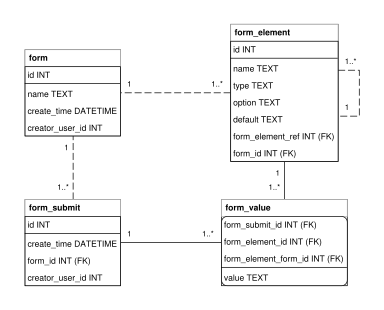
\includegraphics[width=\textwidth]{figures/eer-form.pdf}
    \caption{表单实体\label{DatabaseEntityForm}}
  \end{center}
\end{figure}

表单项(Form Element) 有如下几种类型~\footnote{表单项类型为类型标识符字符串,由应用逻辑定义并进行解释,数据库仅存储类型标识符与字符串值。}:

\begin{itemize}
  \item 隐藏域(Hidden)
  \item 文本域(Text Input)
  \item 文件域(File)
  \item 图片域(Image)
  \item 地址域(Address/Location)
  \item 单选域(Radio)
  \item 多选域(Checkbox)
  \item 长文本域(Text Area)
  \item 富文本域(Markdown)
  \item 日期域(Date)
  \item 时间域(Time)
  \item 日期/时间(DateTime)
  \item 音频(Audio)
  \item 视频(Video)
  \item 用户(User)
\end{itemize}

值得注意的是 $form\_element$ 定义中包含到 $form\_element$ 的外键用于处理 CheckBox、RadioBox、Selector 等的数据源请求。

\subsection{标签/域模式}

为了解决一系列实体的“搜索”问题(如可见性控制、批量操作),设计标签(Tag)机制给每个可检索实体赋予一组标签。

\begin{figure}[!h]
  \begin{center}
    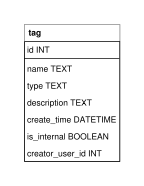
\includegraphics[scale=1.3]{figures/eer-tag.pdf}
    \caption{标签实体\label{DatabaseEntityTag}}
  \end{center}
\end{figure}

为实体赋予标签需要在实体与标签之间建立多对多的关系,实体的标签能够通过实体的创建者以及管理员进行维护。

实体也能够通过标签进行有效性验证,通过与标签建立多对多的 $filtering$ 关系即可存储有效性验证数据。

\newpage

\section{服务器接口设计\label{sec:ServerAPI}}

服务器接口(通信协议)基于 REST(Representational State Transfer) 服务风格设计~\cite{fielding2002principled}。

\begin{table}[!h]
  \begin{center}
    \noindent
    \ttfamily
    \begin{tabular}{|c|c|l|}
      \hline
      \textbf{符号} & \textbf{资源名} & \textbf{描述} \\ \hline
      u & user      & 用户          \\ \hline
      p & profile   & 用户资料      \\ \hline
      m & message   & 消息          \\ \hline
      g & group     & 课程组(分类)  \\ \hline
      c & course    & 课程          \\ \hline
      t & task      & 任务          \\ \hline
      f & form      & 表单          \\ \hline
      s & submit    & 提交(填表)    \\ \hline
      a & answer    & 答案(任务提交)\\ \hline
      r & review    & 评价(评分)    \\ \hline
      y & registry  & 注册(选课记录)\\ \hline
      e & session   & 会话          \\ \hline
    \end{tabular}
    \caption{URI符号表\label{APURIGlossary}}
  \end{center}
\end{table}

\LTXtable{\linewidth}{parts/table/protocol.tex}

上面的表格给出了服务器开放访问的所有数据资源接口以及接口对访问权限的限制,可以看出通过使用 RESTful 的 API 设计风格,通信协议设计可直接对应参照数据库内的实体设计方法,表~\ref{APURIRelation} 给出的接口之间的关系也对应于数据库实体间的关系。

\begin{table}[!h]
  \begin{center}
    \noindent
    \ttfamily
    \begin{tabular}{|c|l|}
      \hline
      \textbf{符号} & \textbf{资源关系描述} \\ \hline
      (u)/(p) & 用户资料     \\ \hline
      (u)/(m) & 用户消息     \\ \hline
      (u)/(c) & 用户的课程   \\ \hline
      (c)/(m) & 课程消息     \\ \hline
      (c)/(t) & 课程任务     \\ \hline
      (f)/(s) & 表单提交     \\ \hline
      (t)/(a) & 任务答案     \\ \hline
      (a)/(r) & 答案评价     \\ \hline
      (c)/(y) & 课程注册申请 \\ \hline
      (y)/(r) & 课程评价     \\ \hline
      (a)-(s) & 答案引用提交 \\ \hline
      (t)-(f) & 任务引用表单 \\ \hline
      (c)-(g) & 课程引用课类 \\ \hline
      (g)-(f) & 课类引用表单 \\ \hline
    \end{tabular}
    \caption{资源关系表\label{APURIRelation}}
  \end{center}
\end{table}

另外,客户端在访问服务器枚举接口时服务器返回列表内元素的 $id$ 列表,客户端需要对每个元素进行单独访问,这要求客户端有一定的缓存机制作为支持以提升请求性能(或者浏览器支持 HTTP Pipelining 机制)。

\newpage

\section{小结}

本章描述了项目中基于用户需求所进行的系统设计活动:

在系统的体系结构设计当中引入了跨服务器-客户端的 MVVM 模式、确定了轻量服务器的构建模式。

数据库设计遵循关系型数据库设计范式,在保证业务高效和数据一致的前提下为应用层提供了良好的数据可扩展性。

使用 REST 风格制定的服务器接口与数据库设计呈现出高度的一致性。

下一章节将对 ViewModel 与 FRP 做出详细的讨论,导出在对交互实现起到重大作用的 ViewModel 构建方式。


\chapter{MVVM 模式与 Reactive Programming}

前三章介绍了项目的背景、需求以及基本的概要设计,本章将着重介绍围绕 MVVM 模式进行的分析与设计活动。

本章将用一定的篇幅详细介绍 MVVM 模式在面向对象的命令式编程语言内的设计实现。使用实例解释 Reactive Programming 以及 FRP 的特性,并导出基于 Reactive Programming 模式的 ViewModel 实现方案。

\section{用户交互与异步编程模型}

用户与计算机的交互是基于人机交互界面(UI)进行的,早期的终端用户界面 (Console User Interface, CUI) 程序与用户进行同步交互,交互的模型为: 用户输入-程序执行-程序输出-用户输入\ldots,这样的逻辑在面向过程编程的语言实现中是非常自然的程序表达——按先后顺序执行每一条语句。

在图形界面(Graphical User Interface, GUI)得到应用之后,用户可以不间断地与程序进行交互而不需要等待程序的执行,这样的设计极大的提升了用户体验。现代的 GUI 程序广泛使用了事件模型处理用户交互,事件是一组时间顺序的离散数据的集合,对程序来说事件是一类异步产生的数据,因此,基于事件进行编程便成为了进行用户交互实现的基本方法。

明确了这点之后,我们可以将行用户交互实现的本质问题归结为~\textbf{处理异步事件}。

基于事件的开发并不是命令式(Imperative)编程模式所擅长的领域,也导致了许多 GUI 程序的交互实现部分都极其不易维护。

以 Drag'n'Drop (拖放操作, DnD) 为例\cite{Zhao2010},在 GUI 上实现 DnD 操作需要程序监听三个不同的 GUI 事件:

\begin{itemize}
  \item 在 MouseDown 事件中标记 isDragging (正在拖动)
  \item 在 MouseMove 事件中判断 isDragging 并且开始绘制拖放光标、使用 API 获取拖放的数据
  \item 在 MouseUp 事件中判断 isDragging 并结束拖放状态(停止绘图)
\end{itemize}

在命令式编程语言中往往使用回调函数(Callback Function)对事件进行处理,这种离散的逻辑碎片导致了在 GUI 实现中出现大量的碎片代码以及全局状态,破坏了“代码逻辑局部性”、“变量局部性”等有利于代码组织和维护的性质。

下面几个小节将就异步编程模型问题对 MVC 与 MVVM 框架进行讨论。

\section{MVC 架构模式}

MVC 架构模式中系统被分成 Model(模型)、View(视图)、Controller(控制器) 三个部分(如图~\ref{PatternMVC})

\begin{figure}[!h]
  \begin{center}
    \includegraphics[scale=0.5]{figures/pattern-mvc.pdf}
    \caption{Model-View-Controller 模式\label{PatternMVC}}
  \end{center}
\end{figure}

\begin{itemize}
  \item \textbf{Model} 处理数据和业务操作
  \item \textbf{View} 负责控制 Model 的显示逻辑
  \item \textbf{Controller} 响应用户事件、更新 Model
\end{itemize}

除了将应用程序划分为三种组件,MVC 模式还定义了组件之间的相互作用。

\begin{itemize}
  \item Model 封装与应用程序的业务逻辑相关的数据以及对数据的处理方法。“模型”有对数据直接访问的权力,例如对数据库的访问。“模型”不依赖“视图”和“控制器”,但模型中数据的变化一般会通过一种刷新机制被公布。为了实现这种机制,用于监视模型的视图必须在模型上注册,从而了解在数据模型上发生的改变。
  \item View 能够实现数据有目的的显示,在视图中一般没有程序上的逻辑。为了实现视图上的刷新功能,视图需要访问它监视的数据模型,因此应该事先在被它监视的数据那里注册。
  \item Controller 起到不同层面间的组织作用,用于控制应用程序的流程。它处理事件并作出响应。“事件”包括用户的行为和数据模型上的改变。
\end{itemize}

直接应用 MVC 模式处理异步逻辑~\footnote{实现上文的 Drag'n'Drop 例子} 非常容易出现下面这样的 Controller 逻辑:

\begin{verbatim}

        boolean isDragging;

        view.on('mousedown', () => {
          isDragging = true
          setPointerIcon()
        })

        view.on('mouseup', () => {
          isDragging = false
          setPointerIcon()
          handleDnD()
        })

        view.on('mousemove', () => {
          if (isDragging) {
            drawEffect()
          } else {
            doSomething()
          }
        })

\end{verbatim}

上面的示例存在两个问题:

\begin{itemize}
  \item 依赖“全局状态”
  \item 本应连续的逻辑被分散到了几个代码块中
\end{itemize}

在软件质量标准中”局部性“ (Locality) 是判断可维护性的一个重要标准。代码的局部性表现在数据局部性与逻辑局部性上,对全局状态的依赖将破坏数据局部性,而逻辑碎片则导致了逻辑局部性的缺失。

当然,这一种实现只是 Controller 对异步逻辑实现中最糟糕的例子。MVC 设计模式并没有对这一部分的逻辑进行更加详细的设计,因此,在 MVC 设计模式的基础上 Microsoft 提出了基于观察者模式 (Observer Pattern) 的 Controller 实现,也就是下文将讨论的 MVVM 模式。

\section{面向对象的 MVVM 实现}

MVVM 模式是对 MVC 模式的一种特殊形式:

\begin{figure}[!h]
  \begin{center}
    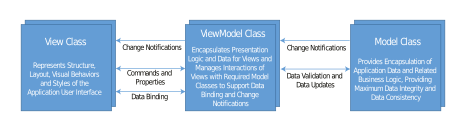
\includegraphics[width=\textwidth]{figures/reference-mvvm-core-classes.pdf}
    \caption{MVVM 设计模式的核心对象\label{MVVMCoreClasses}}
  \end{center}
\end{figure}

图~\ref{MVVMCoreClasses}~\cite{ghoda2012windows} 详细描述了 MVVM 架构中各个组件所负责的任务以及之间的交互关系,其中 ViewModel 在 View 与 Model 中间进行数据处理、转换,是 MVVM 模式中的重要角色。

MVVM 结构中的基本交互:

\begin{itemize}
  \item ViewModel 通过监听 Model 变更对 View 进行更新
  \item View 通过 ViewModel 将用户事件转换为 Model 数据、对 Model 进行更改。
\end{itemize}

Model 与 ViewModel、View 与 ViewModel 之间的通信由 Binder 机制实现。Binder 机制是 MVVM 的 WPF 实现内隐含的设计~\footnote{MVVM 的命名并没有表现 Binder 机制},通过 Binder 实现 ViewModel 到 View 的属性绑定和 ViewModel 对 Model 的监听~\cite{Likness2010}。

在概述中我们也提到 MVVM 架构设计的一个亮点在于 ViewModel 在行为上与 Model 保持的一致性,因此 ViewModel 之间的通信也是通过 Binder 进行的。

在面向对象的设计模式中容易发现观察者模式(Observer Pattern)是非常适合这种场景的。因此,WPF 中使用的 ViewModel + Binder 借口就派生于观察者模式。

\begin{figure}[!h]
  \begin{center}
    \includegraphics[width=\textwidth]{figures/pattern-observer.pdf}
    \caption{类图: 观察者模式\label{PatternObserver}}
  \end{center}
\end{figure}

程序需要先将观察者实例注册至 Subject (被观察者),当 $Subject$ 的属性发生变更时 $notifyObserver$ 方法将得到触发,$notifyObserver$ 将枚举当前注册的所有 $Observer$ 实例并向其推送数据。

参照图~\ref{PatternObserver}~\footnote{Wikipedia: File:Observer.svg} 中的定义对 Model 与 ViewModel 进行定义:

\begin{verbatim}

        @interface IModel implements ISubject;
        @interface IViewModel implements IObserver;

\end{verbatim}

在 MVVM 模式中 ViewModel 作为 Model 的观测者,因而 Model 实现 Subject,而 ViewModel 实现 Observer。

为了让 ViewModel 具有与 Model 相似的行为,将 ViewModel 的接口改写为:

\begin{verbatim}

        @interface IViewModel implements IObserver, IModel;

\end{verbatim}

\begin{figure}[!h]
  \begin{center}
    \includegraphics[scale=0.6]{figures/class-viewmodel.pdf}
    \caption{类图: ViewModel 设计\label{ViewModelClass}}
  \end{center}
\end{figure}

ViewModel 通过订阅 Model 获取 Model 的数据变更(图~\ref{MVVMCoreClasses} 中 Model 至 ViewModel 的 $Change Notifications$)。与之类似,View 与 ViewModel 之间的 Binder 定义:

\begin{verbatim}

        @interface IBinder implements ISubject, IObserver;

\end{verbatim}

Binder 实例构造时指定 View 元素作为 Observer 实例,指定 ViewModel 元素作为 Subject 实例就可以建立 ViewModel 至 View 的单向绑定关系。双向绑定关系由两个单项绑定构成,不加赘述。

值得一提的是,由于 ViewModel 同时实现了 Model 接口,具备了 Model 的行为特性,ViewModel 之间也是可以互相观察的(图~\ref{ViewModelCascading})。

\begin{figure}[!h]
  \begin{center}
    \includegraphics[scale=0.6]{figures/class-viewmodel-cascading.pdf}
    \caption{类图: ViewModel 级联设计\label{ViewModelCascading}}
  \end{center}
\end{figure}

这样的设计使得 ViewModel 模式获得了很强的可扩展性,将用户交互状态分开给不同的 ViewModel 进行管理可以显著减小业务逻辑状态的维护难度,开发者可以利用封装的 ViewModel 类库进行组合来完成用户交互逻辑的实现,具有很高的可复用性。使用 ViewModel 进行开发也同时带来了良好的可测试的代码结构。

上节我们已经看到直接使用回调函数实现 Controller 处理异步交互事件的弊端,在使用使用观察者模式(Observer Pattern)、利用观察者响应事件数据的 MVVM 模型中 Drag'n'Drop 逻辑的接口实现是这样的:

\begin{verbatim}

        @class DnDObserver implements IObserver
          @state  boolean isDragging;
          @state  Coord   prevCursorPosition;
          @method void notify (propName, oldValue, newValue);

        @interface ObservableView implements ISubject

\end{verbatim}

上面的代码通过使用 $DnDObserver$ 封装 $isDragging$ 状态从而解决全局状态依赖的问题,在 $notify$ 函数内集中实现拖放的业务逻辑可以解决代码逻辑碎片化问题。另外,封装完好的 $DnDObserver$ 还可以被方便的复用到其他 View 之上。

$ObservableView$ 将事件抽象为一系列数据以及对属性变更事件的触发,$DnDObserver$ 监听 $ObservableView$ 的属性变更,这样的实现维护方便、有较强的可复用性。

MVVM 模式通过结合 MVC 架构与 Observer 模式优化了面向对象编程语言环境下事件驱动的用户界面开发模型,即,MVVM 模式是 MVC 模式在处理异步编程模型场景下的一种特殊形式。而在异步事件的处理方面,声明式(Declaritive)语言的表述却显得更加自然,使用声明式风格进行用户交互实现的尝试也越来越多。下一节将引入 Reactive Programming 在异步事件处理方面就有非常出色的性能。

\section{Reactive Programming 与 Monad 函数}

Reactive Programming 的概念继承自 FRP,随着越来越多的语言融入和函数式语言的开发方法,Reactive 模式也被越来越多的应用在 GUI 应用开发当中~\footnote{http://www.reactivemanifesto.org/}。

Reactive Programming 是一种声明式的开发方法,用户通过声明数据的“转换”对系统行为进行建模(描述“是什么”)。相对的,命令式编程范型(Imperative Programming Paradigm)中,开发者需要对系统的每一步行为进行描述(描述“如何做”)。

当然,声明式编程范型在描述具体的系统行为方面并没有优势(如 Haskell 中就使用 $do$ 语法糖模拟命令式范型),因此,还是需要通过命令式编程范型对程序行为进行细节描述,这部分的描述具有很高的抽象程度和可复用性,在拥有足够多的行为定义以后就可以完全通过声明对系统进行建模了。

也由于上面介绍的这一特性,Reactive Programming 在 JavaScript 这样支持函数式编程方法的命令式编程语言中能够得到很好的实现~\footnote{类似的语言平台还有 C\#、Scala 等}。以 Reactive.js~\footnote{此处使用的是 Reactive.js 的最小 Reactive 核心} 为例~\cite{Carkci2013}

\begin{verbatim}

        // Declaration
        var A = $R(function (b, c) { return b + c });
        var B = $R.state(2); // Initial value for B
        var C = $R.state(1); // Initial value for C
        A.bindTo(B, C); // Declare B and C as argument for A

\end{verbatim}

上面的代码片段演示了 $A = B + C$ 的 Reactive 定义(使用 JavaScript 语言环境),当更改 $B$ 或 $C$ 的值发生改变时 $A$ 的值便会“自动”进行重新计算:

\begin{verbatim}

        // Reaction
        A();   // -> 3
        B(5);  // Set B to 5
        A();   // -> 6

\end{verbatim}

FRP 的将系统抽象为行为(Behaviors)和事件(Events),上例中先使用 Monad 函数包装行为(见 A、B、C 的定义)并在行为之间建立关联(上例中使用 $bindTo$),然后通过传入事件($B(5);$) 更改“行为”的值。

Reactive 定义中出现的 $\$R$ 函数所产生的对象(即 A、B和C)与 Haskell 中为 Monad 拥有相同的定义~\cite{raey},$\$R$ 即 Monad 构造器,后文中使用 Monad 指代这类对象。

Monad 在形式上是一个”数据“而实现上是一个封装了“计算”的高阶函数,FRP 的定义中 Monad 就是所谓的行为(Behavior)。在命令式语言中实现的类 Monad 高阶函数通过“缓存”依赖数据的形式,以使逻辑脱离上下文依赖。

不难发现,Monad 与 Observer 有非常相似的行为:

\begin{itemize}
  \item 需要对监听/绑定关系作出声明
  \item 在发生变化时对变化做出响应
\end{itemize}

Monad 与 Observer 之间的区别是 Monad 通过包装数据实现监听而 Observer 通过让数据模型实现接口。相比 Observer,Monad 的使用更加灵活(可以应用于任何粒度的数据),而 Observer 则更具有扩展性。

受到 Reactive.js 的启发,项目中定义了 Monad 作为 Reactive 的核心结构:

\begin{verbatim}

        @interface Monad
          @method [Any] get (default: Optional-any)
          @method [Monad] set (new_val: Any)
          @method [Monad] on (event: Value-in('get', 'set'))
          @method [Monad] setup ()
          @method [Monad] teardown ()

\end{verbatim}

\begin{itemize}
  \item 使用 $get$ 方法获取 Monad 包装的数据
  \item 使用 $set$ 方法给 Monad 赋值,同时触发赋值事件
  \item $on$ 接口为 Monad 绑定事件(定义具体操作)
  \item $setup$ 与 $teardown$ 用于控制消息传递的开始和结束
\end{itemize}

这样定义以后在程序中实现 Drag'n'Drop 逻辑只需声明:

\begin{verbatim}

        dnd(mousedown(view), mouseup(view), mousemove(view))

\end{verbatim}

$mousedown$、$mouseup$ 与 $mousemove$ 函数分别产生 $view$ 对应事件对象的 Monad 高阶函数,$dnd$ 函数控制 Drag'n'Drop 过程中的程序动作~\footnote{dnd 过程使用命令式进行定义}。

这里需要注意的是 $dnd$ 是一个返回 Monad 函数的高阶函数,接受三个 Monad 函数作为参数,通过 $on$ 方法监听三个 Monad 函数参数的变更,实现 FRP 中的 Pull 传递模型~\cite{Elliott:2009:PFR:1596638.1596643}。

\section{小结}

异步编程模型是在进行图形用户界面程序设计与开发过程中非常重要的一部分,不难发现解决交互开发问题的关键在于合理的组织代码处理异步事件。在 FRP 平台中,异步事件处理逻辑得到很自然的表述~\cite{Wan:2002:EF:645772.667941},Microsoft 推出的 F\# 也将事件作为一等对象提出了类似的异步事件开发模型~\cite{Syme:2011:FAP:1946313.1946334}。异步事件处理模型已经由最开始的面向过程的回调函数演化到了一种语言模型,本项目也正是在这些工作的基础上,结合 JavaScript 平台的语言特性对 API 进行合理设计。

本章作为本文讨论的重点之一,讨论分析了图形用户界面开发的本质问题——异步编程,说明了 MVC 架构与 MVVM 架构的关系。使用实例讨论了面向对象 MVVM 模式实现的基础——Observer 模式,说明了 Observer 模式在处理异步事件方面所具有的优势。

本章还通过实例分析了 Reactive Programming 的应用,说明 Monad 与 Observer 的行为相似性,并引入了本项目中使用的 Reactive 核心接口。


\chapter{实现}

本章整理总结系统实现过程中遇到的关键问题的解决方案以及解决问题的过程中进行的探索性过程。\footnote{考虑到表述紧凑性,本章节仅包含描述解决方案所必须的代码片段,详细的代码实现请参考附录内的相关内容}

\section{开发环境与技术选择}

系统开发主要使用 JavaScript 语言平台,应用服务器端使用 Node.js 而客户端使用 JavaScript 脚本开发业务代码。

\begin{figure}[!h]
  \begin{center}
    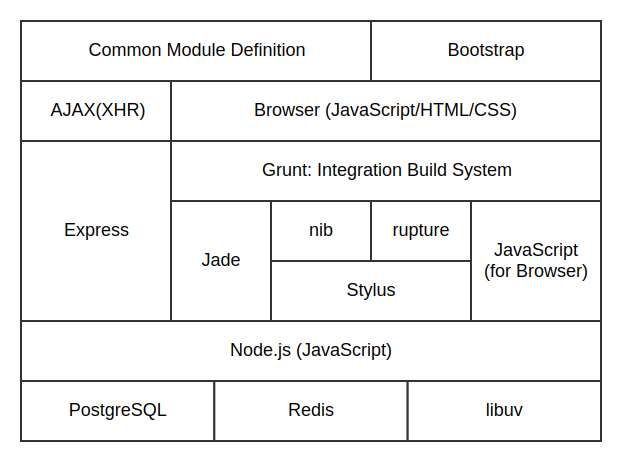
\includegraphics[width=\textwidth]{figures/techstack.pdf}
    \caption{开发环境与外部组件\label{TechStack}}
  \end{center}
\end{figure}

相较 Java/.NET 等流行的企业级解决框架,Node.js 支持函数式编程范式,在 Express 框架的帮助下可以快速的搭建稳定的服务器应用。另外,选择 Node.js 的一大原因是 Node.js 采用消息队列机制,并支持异步 I/O 操作,单线程异步操作模型可以有效的减少内存开销,同时,避免了传统服务器开发过程中所容易出现的线程同步问题,极大的提升了服务器的稳定性。对轻量服务器设计来说使用 Node.js 能够在取得良好的服务器性能以及稳定性的同时达到最大的开发效率。

客户端代码使用 Grunt 集成编译系统进行独立编译,相比使用 Express 进行线上编译-缓存的策略,使用 Grunt 集成编译环境直接将客户端程序编译为线上版本有利于前端服务器直接对文件进行缓存操作,将客户端资源编译工作从应用服务器中分离出来也有利于应用服务器自身的可扩展性和运行时性能。

\section{服务器(Model)}

应用服务器的职能在系统中主要负责多用户会话维护、权限控制以及数据操作。

\subsection{轻量级 Object-Relation Mapping 实现}

Object-Relation Mapping (ORM) 是将数据库关系与数据库实体的数据直接通过面向对象封装进行访问的一种方法。

服务器对数据库的业务访问逻辑普遍包含:

\begin{itemize}
  \item 验证业务数据有效性
  \item 转换业务数据(如 进行 Password Hash)
\end{itemize}

为了提高数据库访问代码的复用程度,项目中设计了 $querybuilder$ 轻量级数据库 ORM 框架,以用户资料管理为例:

\begin{verbatim}

        profile: {

          update: qb('INSERT INTO profile SET ? ON DUPLICATE KEY UPDATE ?', {
            user_id : Number,
            name    : String,
            gender  : String
          }),

          query: qb([
            'SELECT a.`user_id` AS `user_id`,',
            '       p.`name`    AS `name`, ',
            '       p.`gender`  AS `gender`,',
            'FROM `account` a INNER JOIN `profile` p ON a.user_id = p.user_id',
            'WHERE a.`account` = :account AND a.`domain` = :domain'
          ].join(' '), { account: String, domain: String })

        },

\end{verbatim}

$qb$ 函数返回用于数据库查询的高阶函数,在中间件中:

\begin{verbatim}

        db.profile.update(req.data, function (err, result) {

          if (err) {
            return next(new ApplicationError({
              message: 'Failed to update user profile',
              cause: err
            }));
          }

          return res.status(200).end();

        });

\end{verbatim}

通过使用简单的 ORM 框架,对 SQL 语句模板进行集中统一的管理,让业务逻辑代码得到了高效的组织。

\subsection{权限控制中间件}

中间件是 Express.js 服务器框架所使用的基本设计模式。

\begin{figure}[!h]
  \begin{center}
    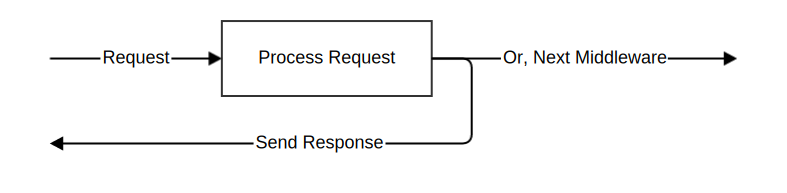
\includegraphics[width=\textwidth]{figures/pattern-middleware.pdf}
    \caption{中间件行为示意图\label{ExpressMiddleware}}
  \end{center}
\end{figure}

获得请求以后 Express.js 会按照中间件的注册顺序使用中间件处理请求,中间件返回三种处理结果:

\begin{enumerate}
  \item 处理完成,发送响应数据
  \item 进行数据变换,发送至下一个中间件
  \item 处理失败,使用错误处理中间件进行处理
\end{enumerate}

权限控制中间件用于实现服务器接口的权限控制(见~\ref{sec:ServerAPI})。

权限控制中间件通过传入的高阶函数判断当前对接口进行的请求的合法性:

\begin{verbatim}

        app.post('/c/:id/t/',
          // role of current user is admin or teacher
          accessctl(role('admin'), role('teacher')),
          // can access c of :id with current request
          accessctl(from('/c/:id/', 'c')),
          function (req, res, next) {
            // Bussiness code
          }
        )

\end{verbatim}

上面的例子中 $role$ 与 $from$ 分别是用于确认用户角色以及其他接口访问能力的~\textbf{权限策略},$accessctl$ 通过执行权限策略并检查策略的执行结果决定是否给予当前的请求进行下一步中间件。

除了应用于对某个接口的权限控制,$accessctl$ 还可以通过 $express.use$ 方法配置一组 $router$ 的权限。

\section{客户端视图模型(ViewModel)}

项目中使用 Monad 对 MVVM 模式中 ViewModel 进行实现,替代面向对象设计中的 Observer 模式。Monad 与 Observer 都能合理的组织代码,将代码复杂度保持在线性增长的状态,而 Monad 在函数式开发环境中更容易实现和使用。

本项目尝试开发的 Entangle 框架经过三次迭代最终满足客户端前端开发的需求,Entangle 框架使用 Monad 作为 Reactive Programming 的响应核心,并在此基础上封装 Builder 模式以简化对业务逻辑中经常出现的顺序逻辑的定义过程。下面几个小节对 Entangle 框架成型过程中所解决的重要业务需求以及其实现方案进行叙述。

\subsection{数据同步}

与服务器进行数据交互是客户端的基础功能之一。

通过 $http$ 转换子(Converter)实现从服务器拉取数据:

\begin{verbatim}

        entangle().http('GET', '/u').pick(function (data) { /* ... */ });

\end{verbatim}

Entangle 使用链式表达式构建串行关系的转换子(Converter),上例实现获取用户信息的功能。

对于轮询的情况,可以使用 $timeout$ 转换子:

\begin{verbatim}

        var juice = entangle().http('GET', '/u')
        var timer = entangle().timeout(2000);

        timer.fork(juice);
        juice.fork(timer);

\end{verbatim}

$fork$ 原语将 timer 的值转发到 juice,当 timer 触发时,触发事件会传递给 juice、发出 http 请求,请求完成后 juice 又会将数据 fork 回 timer 进行下一个 $2s$ 的等待。这样就造成了一个轮询的数据流。

详细的实现请参考附录内容,在这里我们不详细展开 Entangle 的实现细节。

\subsection{页面导航}

页面导航栏的逻辑是单一对象数据绑定的比较典型的实现。entangle 通过自动改写的 jQuery 方法实现对用户界面元素的操作,下面这些代码来自 pilot.js:

\begin{verbatim}

        entangle()
        .location()
        .pick().string('.navbar-collapse a[href="{{pathname}}"]')
        .$().$parent('li').$addClass('active')

\end{verbatim}

$string$ 转换子将输入的数据代入字符串模板,$\$$ 转换子将输入的字符串转换为 jQuery 对象之后以 \$ 开始的转换子都经过自动改写指向对应的 jQuery 方法。

$location$ 转换子实现对页面地址信息的监听:

\begin{verbatim}

        location: function () {

          var converter = function () {
            this.resolve(location);
          };

          // get location from window object
          var location = {
            host: window.location.host,
            hostname: window.location.hostname,
            protocol: window.location.protocol,
            search: window.location.search,
            href: window.location.href,
            port: window.location.port,
            pathname: window.location.pathname,
            hash: window.location.hash,
          };

          // listen for hash change event
          $(window).on('hashchange', function () {
            location.hash = window.location.hash;
            converter.resolve(location);
          });

          return converter;

        }

\end{verbatim}

这里介绍一下转换子的构成:

\begin{itemize}
  \item 转换子是一个返回高阶函数的函数
  \item 转换子内可以定义自己的闭包状态
  \item 转换子可以进行事件监听
  \item 转换子使用 $resolve$ 方法将数据传输给后继转换子
\end{itemize}

另外,这里需要特别说明的问题是,基础的转换子实现是基于面向过程的编程方法的,事实上 Haskell 在描述具体的“怎么做”(HOW)逻辑的时候也使用 $do$ 语法糖模拟顺序执行的代码(通过参照代码行之间的前后依赖关系,在定义“是什么”(WHAT)的情况下依赖关系是由“是什么”定义的,不参照代码行的前后依赖关系),这也是支持混合语言特性的语言的优势所在。

\subsection{绑定列表数据}

第三版的 entangle 对列表数据的绑定做出了设计,第二版 entangle 中使用 entangle 核心对上下文进行切换管理,这样做所产生的代价是核心代码的大量冗余与不可扩展性,因此,第三个版本的 entangle 采用了 monad 的封装机制,仅实现最核心的 Reactive 需求。在做出了这样的修正之后,编写清晰的列表数据的绑定逻辑成为可能。

\begin{verbatim}

        init: entangle().json('get', '/c/').pick('data')

\end{verbatim}

首先,$init$ 从服务器获取对象 id 列表,然后 id 列表数据被传送到 $list$ 进行扩展:

\begin{verbatim}

        list: entangle().collect(_.identity).each(function () {
          // return [Entangle Object]
        })

\end{verbatim}

为了处理列表数据条目的增加与删除,我们需要从列表项中提取出没个项目的唯一 id,并构造字典,这一工作由 $collect$ 转换子完成。

接下来将整个列表传入 $each$ 转换子,$each$ 转换子接受一个产生转换子的函数作为参数(factory 函数),$each$ 转换子内部会为不同的元素分别调用 factory 函数产生对应的转换子,由产生的转换子管理子元素的状态。

特别地,转换子内需要判断转换子所管理的元素是否已经被删除。

\subsection{数据缓存与按需触发}

性能因素是 FRP 的缺点之一~\cite{Elliott:2009:PFR:1596638.1596643},对计算结果做缓存以及按需触发控制能够有效的减小性能开销。

entangle 设计了 $sponge$ 用于缓存输入的数据结果与控制触发信号的输出。

\begin{verbatim}

        entangle()
        .string('/u/0/p').json('get').pick('data')
        .sponge()
        .$('.view-photo-img').$attr('src', '{{photo}}')

\end{verbatim}

此处设置了 $sponge$ 转换子,则在用户资料没有发生改变的情况下不通知 $\$('.view-photo-img')$ 对象改变其 src 属性

$sponge$ 转换子提供 $alwaysTrigger$ 参数来配置触发行为,若使用 $sponge(true)$ 则后继转换子不论 sponge 内的缓存是否更新都会得到触发信号。

\subsection{代码调试工具和策略}

在设计 entangle 的 API 的过程中进行了许多的调试工作,在异步编程的环境下进行调试无法像在同步环境内进行单步跟踪那样对异步代码进行切实的跟踪。异步代码的“单步”调试的实现要依靠调试人员在调试时人工进行动态的断点调整来实现,这也是极其麻烦的一项工作。

为了使用户能够方便的调试 entangle 数据流,entangle.debug 函数集包含了 entangle.logger 和 entangle.breakpoint 转换子,这些转换子不会影响业务数据的传递,entangle.logger 会在 console 输出到达的数据而在程序执行到 entangle.breakpoint 时会提示调试器进行中断,以方便调试人员找到异步事件的调试入口。

虽然这些调试机制还不是相当完善,在一定程度上辅助以适当的调试策略还是能够取得非常良好的调试效果。

\section{客户端视图(View)}

View 的开发使用了 Jade(HTML预处理器) 和 Stylus (CSS预处理器) 组合。使用预处理器进行视图开发有下面几个优势:

\begin{itemize}
  \item 代码冗余度低
  \item 视图元素/样式复用
  \item 模块化视图开发
  \item 可实现简单视图逻辑
\end{itemize}

\begin{figure}[!h]
  \begin{center}
    \includegraphics[scale=0.3]{figures/screenshot/enroll.png}
    \caption{学员录取视图\label{SSEnroll}}
  \end{center}
\end{figure}

\begin{figure}[!h]
  \begin{center}
    \includegraphics[scale=0.3]{figures/screenshot/userman.png}
    \caption{用户管理视图\label{SSUserMgr}}
  \end{center}
\end{figure}

\begin{figure}[!h]
  \begin{center}
    \includegraphics[scale=0.3]{figures/screenshot/review.png}
    \caption{课程评分视图\label{SSCourseReview}}
  \end{center}
\end{figure}

\begin{figure}[!h]
  \begin{center}
    \includegraphics[scale=0.5]{figures/screenshot/responsive.png}
    \caption{用户管理视图(移动终端)\label{SSResponsive}}
  \end{center}
\end{figure}


\chapter{总结与展望}

关于系统设计及实现至此就全部阐述完成了,在系统设计过程中遇到许多设计困难,在设计方面做了许多尝试、走了不少弯路。本章对整个毕业设计的过程、毕业设计的过程中所出现的各种问题做一个总结。另外,本章还对将来的一些研究做出一些展望。

\section{MVVM架构与Reactive}

由于接触过 WPF 框架下的 MVVM 模式,在开始毕业设计之初的目的就是在 JavaScript 的平台上实现一个 MVVM 框架并进行一次正式的 MVVM 开发实践,随着研究的深入,我对 MVVM 架构的理解也变得更加透彻起来,也认识到 Observer 模式在解决异步编程方面发挥着的重要作用。我个人对于小而美的架构设计有强烈的偏好,所以开始尝试设计一款轻量级的 MVVM 架构应用到项目中。

在函数式语言的领域内我找到了一个答案—— Functional Reactive Programming。后来在研究过程中我发现 Observer 与 Monad 的共同点,而 Monad 所采用的模式能够被 JavaScript 轻易地实现,于是就产生了 Model-View-ReactiveModel 模型(使用 Monad 替代 Observer 的 MVVM 实现)。

在项目中的这个实现命名取自量子纠缠(Entanglement),作为尝试性的实现,entangle 虽然能够达到维护客户端数据的目的,但也还是存在着一些不足。

虽然已经将 entangle 的核心设计减小到了一定的程度,entangle 在 API 的定义上还没有经过梳理,易用性和代码可读性上都不能真正达到产品的标准。

这些不足体现在:

\begin{itemize}
  \item 建立 Monad 之间关系的过程较繁杂
  \item 与外部库对接上存在 API 接口一致性问题
  \item 需要建立命名空间对不同类型的转换子进行分别管理
  \item 内存管理模型不明确,存在一定风险
\end{itemize}

\section{未来的研究方向}

接下来的开发工作希望能够在课程管理系统的实践基础上,将业务逻辑从课程管理延伸到通用 OA 应用领域。

架构研究方面,为了克服上文提到的一些不足,考虑在 JavaScript 的基础上设计或选择一门编译至 JavaScript 代码并且能够与 JavaScript 执行环境进行互操作的函数式语言用于定义 ReactiveModel 以突破 JavaScript 平台的语言限制,使用更简单的形式定义 Monad 之间的关系。另一方面,对内存管理进行研究,增加内存保护提示措施。



%参考文献
\cleardoublepage
\phantomsection
\addcontentsline{toc}{chapter}{参考文献}
\bibliography{IEEEabrv,reference}

%致谢
\cleardoublepage
\phantomsection
\addcontentsline{toc}{chapter}{致\qquad 谢}
\chapter*{致\qquad 谢}
\songti\zihao{-4}

本毕设的完成离不开许多人的帮助,首先我要在此感谢北京邮电大学互联网创新实验室的刘禾刘老师作为我本科毕业设计的指导老师。在刘老师的帮助下顺利地完成了系统的需求分析与设计。互联网创新实验室的创新实验环境也给我的毕业设计带来了很多的创意和灵感。

我还需要特别感谢来自朋友们的帮助和支持。感谢蓝星灿学长帮助我调整论文排版并推荐了 Entanglement 这个名字;感谢李明洋学姐在外文资料词汇翻译方面为我提供的指导和帮助;感谢使用专业知识帮助我解决了许多项目的前端布局实现过程中的问题的 David Clark 先生。最后需要感谢本文 LaTex 模板的作者樊高峰学长以及在精神上给予我极大支持的父母与朱轶伦前辈。



%附录
\cleardoublepage
\phantomsection
\addcontentsline{toc}{chapter}{附\qquad 录}
\chapter*{附\qquad 录}

\section*{附录~1\quad	课程管理系统业务过程模型}
\label{sec:appendix-bpm}

本节为图~\ref{BPMOverview} 提供展开补充。

\begin{figure}[!hbp]
  \begin{center}
    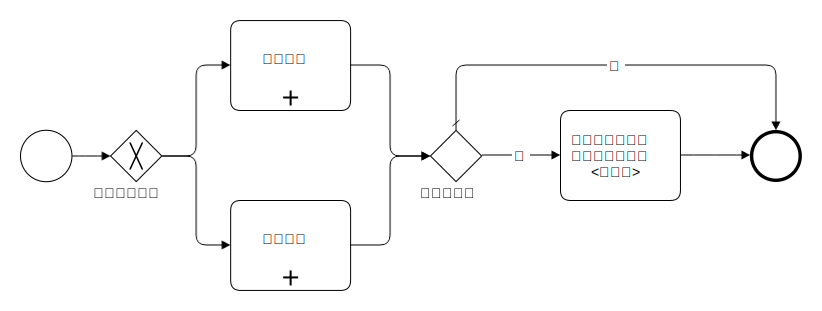
\includegraphics[width=\textwidth]{figures/bpm-cs.pdf}
    业务过程模型示意图(选课)\label{BPMCourseRegister}
  \end{center}
\end{figure}

\begin{figure}[!hbp]
  \begin{center}
    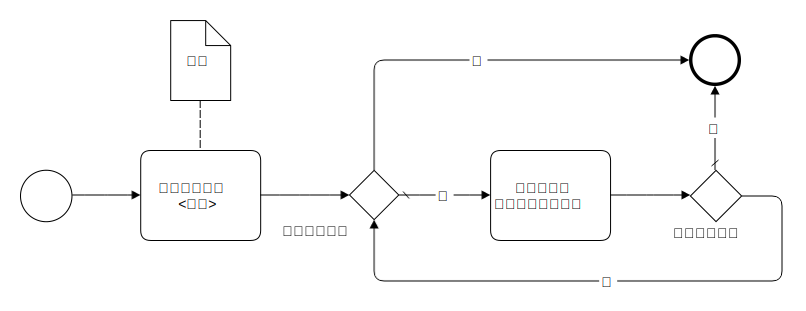
\includegraphics[width=\textwidth]{figures/bpm-cs-pref.pdf}
    业务过程模型示意图(选课-志愿)\label{BPMCourseRegisterP}
  \end{center}
\end{figure}

\begin{figure}[!hbp]
  \begin{center}
    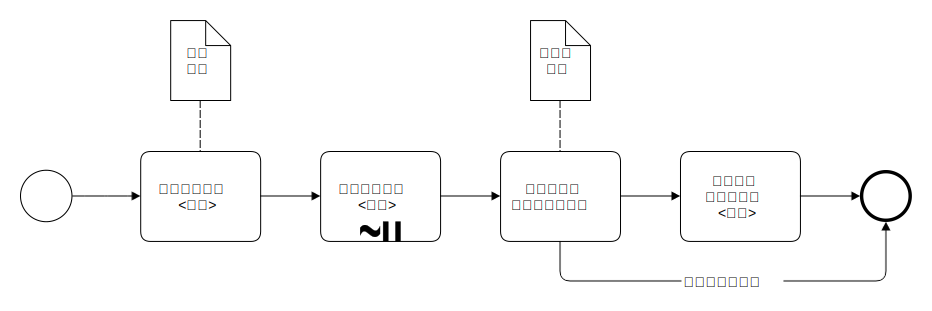
\includegraphics[width=\textwidth]{figures/bpm-cs-dual.pdf}
    业务过程模型示意图(选课-双选)\label{BPMCourseRegisterD}
  \end{center}
\end{figure}

\begin{figure}[!hbp]
  \begin{center}
    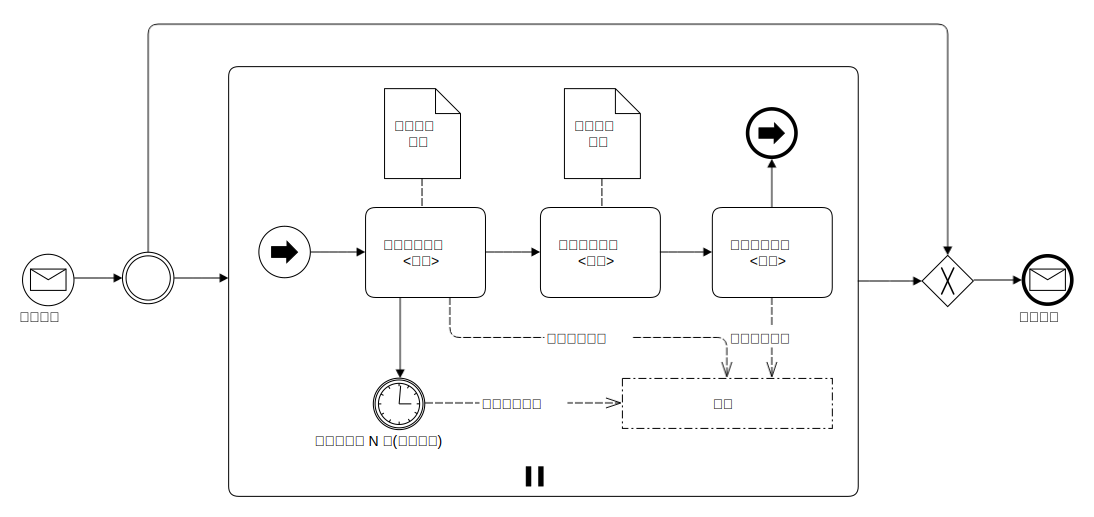
\includegraphics[width=\textwidth]{figures/bpm-task.pdf}
    业务过程模型示意图(课程任务)\label{BPMTask}
  \end{center}
\end{figure}

\newpage

\section*{附录~2\quad	课程管理系统产品需求表格}
\label{sec:appendix-requirement-table}

\LTXtable{\linewidth}{parts/table/requirement.tex}

\newpage

\section*{附录~3\quad	数据库设计示意图}
\label{sec:appendix-database-diagram}

下图展示完整的数据库设计视图:

\begin{figure}[!h]
  \begin{center}
    \includegraphics[angle=90, scale=0.5]{figures/eer-120dpi.png} \\
    数据库设计视图\label{FullDatabaseDesign}
  \end{center}
\end{figure}

\newpage

\section*{附录~4\quad	QueryBuilder 模块实现}

\verbatiminput{parts/code/querybuilder.js}

\newpage

\section*{附录~5\quad	Entangle 核心实现}

\verbatiminput{parts/code/entangle.js}



%清除页眉页脚
\pagestyle{empty}

%外文资料(译文/原文)
\chapter*{外\quad 文\quad 译\quad 文}
\pagestyle{empty}

\begin{center}
{\heiti\zihao{3}HotDrink}

{\heiti\zihao{4}A Library for Web User Interfaces}

\textsl{By John Freeman, Jaakko Järvi, Gabriel Foust}

{\heiti\zihao{3} HotDrink}
\end{center}

\zihao{-4}

\section*{摘要}
HotDrink是一个用于创建表格、对话框以及其他Web应用常用的用户界面组件的JavaScipt库。使用HotDrink,开发者用JavaScript声明了一个“视图模型”,并在模型与组成视图的HTML 元素之间建立一系列的“绑定”。这些规范虽然微不足道,但足够让HotDrink提供一个全功能的GUI,包括多路数据流、启用/禁用数值、激活/无效命令以及数据验证。HotDrink以高质量的用户接口将这些丰富多彩的行为实现为可重用代码。这篇文章以及工具演示通过逐步的展示一个Web应用GUI的构建过程,向开发者介绍HotDrink库。
\section*{前言}
用户界面(UI)编程往往费时费力。有研究表明,创建应用时,UI实现的代码平均占40\%[14],另一个研究为平均30\%[10]. 这些数字很高但可能并不令人惊讶;UI实现往往需要大量的、不可重用的、此应用专属代码。
一个典型的图形UI库提供的主要服务就是将用户行为转化为事件并将事件递交给相应的事件处理函数。UI程序员写出事件处理程序并注册去监听相应事件。这也是目前主要的Web UI编程模型;UI行为在事件处理程序中用程序逻辑定义好。
随着编程社区逐渐接受事件处理程序模型,其他方法已经且正在被寻找。我们定义了两个趋势:(1)用宣告式数据流约束代替命令式事件处理;(2)设计能帮助程序员分离数据展示和逻辑的模式
对第一个趋势,针对UI的数据流约束系统在过去几十年里被积极的研究过[5,13,16],并已经被使用,比如在UI元素的布局与排列中。最近的一些Web编程框架[2,1,3]也使用了约束来管理显示在UI控件中的变量,特别与观察者模式一起[8,5]。
至于第二个趋势,流行的设计模式的发展,从Model View Presenter[15],到Presentation Model[6],到Model View View Model[9],(MVVM), 反应了针对代码分离更好的设计的追求。这些模式中最新的,MVVM,其目标是创建没有逻辑,只需保留从用户行为保留事件、与从视图模型展示数据的任务。视图模型维护UI的状态,也就是与展示在控件上的内容密切相关的、能反应一部分模型数据的数据。模型是应用“业务”数据与逻辑的统一体,和在传统的MVC模式中一样[12]。
为实现宣告式的用户界面编程,HotDrink 采用我们的属性模型方法[10,11,7]。它结合了上述两种趋势:HotDrink中的视图不包含编程逻辑(通常他们只是HTML控件的声明),并且所有的UI状态被包含在一个视图模型中,这个模型被实现为多路数据流约束系统。HotDrink的最终代码简明清晰,因其对编程者隐藏了所有事件处理代码,并且将许多复杂的UI行为(变量传播、控件可用/禁用、命令激活/失活等等)实现为可重用算法
这篇文章/工具演示对HostDrink的主要功能进行了描述。我们将带着读者了解一个Web UI例子的实现的流程,来解释程序员视角——程序员创建一个GUI的时候要写的一系列说明。
最后,HotDrink的设计允许增量采用,如果需要,一部分用户界面可以受HotDrink控制,但另一部直接被JavaScript事件处理函数或其他的GUI框架控制。HotDrink在Object和Array原型上添加了一些方法,但不用担心这些附加会跟其他库冲突。
\section*{例讲程序员视图}
图1显示了典型酒店预订表单的一个部分。预订服务需要入住和离开时间以查询可入住的房间。增加“晚”这个字段之后,该UI提供了三种方法来指定这些日期――通过任意两个字段都能推断出第三个字段的值。我们将介绍如何使用HotDrink及Model-View-ViewModels模式来构造这个界面。读者可到hotdrinkjs.com/date-example下载实现代码。
\begin{figure}[!hbp]
  \begin{center}
    \includegraphics[scale=0.3]{figures/translation/translation_hotdrink_fig1.png}
    选择旅店住宿时段的表格
  \end{center}
\end{figure}
\subsection*{模型}
模型本身是在HotDrink范围之外。对于一个酒店预订应用,它的组成可能会包括一个房间、预订信息数据库以及普通查询的各种算法,比如检查是否有可用房间、增加或删除预订信息。HotDrink假定一个模型已经存在,然后帮助在这个模型之上构建一个用户接口。模型与视图之间的绑定应当由程序员实现,比如在一边移动数据以响应另一边的变化。HotDrink提供视图-模型的更改通知以支持这个任务。
\subsection*{视图-模型}
HotDrink API 提供一种嵌入式特定领域语言(在JavaScript中)来定义视图-模型。在这种语言中,程序员声明变量及它们之间的关系,一起组成这个视图-模型的约束Constraint系统。
所有API存在于hd命名空间。图2显示了酒店预订表单视图-模型的API规范。
\begin{figure}[!hbp]
  \begin{center}
    \includegraphics[scale=0.3]{figures/translation/translation_hotdrink_fig2.png}
    表格的视图模型
  \end{center}
\end{figure}
变量可赋予值。直接不加参数地使用这个变量可获得它的值,重新赋值时可将新值作为唯一的参数。图2所示的例子中有三个变量:分别为住几晚的数目、入住时间、离开时间。每个变量存储一个整数。两个日期变量以Unix epoch以来的毫秒表示。前两个变量以传递给hd.variable的值来初始化。在视图-模型的第一次更新(以下会介绍)时,最后一个变量由前两个变量得到初始化。
Constraints表达了变量之间的关系。每个Constraint由一组方法组成,每个方法是一个满足该Constraint(约束)的过程,――比如建立关系――使用其它变量作为输入,计算某些Constraint的变量的新值。在我们的例子里,唯一一个Constraint的声明开始于第5行,指定了三个方法。每个方法定义列出了它输出的一组变量,并以一个未命名的函数定义了这个方法的过程。
HotDrink要求程序员显式地指定一个Constraint的每个方法。对于某些关系,比如简单的相等,它有可能能够导出所有的方法,但这一点并不是对所有关系有效。将一个Constraint的变量划分成输入和输出组的每一次划分都定义了一个direction,并且,不是所有的direction都可能有关系, e.g., a one-way hash。
变量和Constraint一起组成了多向数据流Constraint系统。实现一个Constraint系统就是执行每个Constraint的一个方法,并且执行顺序不得使之前所满足的Constraint无效。在本文的其它地方我们对此进行了详细的介绍。
更新视图-模型(view-model) 实现了Constraint系统,并对于所有变量的变化发出了通知。增加一个变量或Constraint,写一个变量或显示的调用hd.update会引发一次更新。接受该通知的事件处理器将处理由view-model对model带来的响应,如上所述,并将处理由view-model对view带来的响应,如下所述。
HotDrink支持潜在Constraint系统的增量构造――可对已经与view绑定的系统增加新的变量和Constraint――这将允许view-model根据用户需求变化。
\subsection*{视图}
View和model一样,位于HotDrink的范围之外。View可由标准的HTML元素或者第三方widget工具包构造。我们的酒店预订表单的view是用Html写的,如图3所示。
\begin{figure}[!hbp]
  \begin{center}
    \includegraphics[scale=0.3]{figures/translation/translation_hotdrink_fig3.png}
    图1旅店预约表格的视图元素
  \end{center}
\end{figure}
Binding处理了widgets中view与view-model的变量之间的数据交换。它们可以是单向的(从view-model到view),或者是双向的。HotDrink为从views到view-models之间的binding提供了两种机制:javaScript或者Html属性。我们的例子选择了声明性binding,如图3所示。
Binder是一个函数,用来构造和注册一个事件处理器,后者实现某个特定的binding。比如,HotDrink文本binder将一个HTML文本输入widget与view-model的一个变量绑定,使用了两个事件处理器:
\begin{itemize}
  \item第一个监听widget的变人,并写入变量
  \item第二个监听变量的变化,并更新widget
\end{itemize}
事件处理器是如此的琐碎,因为view-model constraint 系统处理了UI数据之间的所有依赖。在view出现变化的情况下,第一个处理器为constraint系统的一个变量分配一个新的值,引发一次更新。在solve 了constraint系统之后,view-model通知第二个处理器它所负责的widget或许需要更新。
Binder包装了很多细节,包括观察view中的变化,更新view,以及将view中所使用的数据类型转换为view-model所使用的数据类型(反之亦然)。可以自定义binder来扩展hotdrink以支持任何view。在简单的情况下,binder只需要几句代码即可。HotDrink为标准的HTML widgets提供了内建binder。
构建binding时将一个widget和一组选项传递给一个binder。为了方便,binding可以在HTML中使用data-bind属性声明。这个属性是一个JSON对象,其键为binder名字,其值为binder选项。当指向成功,HotDrink用widges和配置数据调用各个已命名的binder。在构建复杂的binding时,比如为第三方使用javascript的jwidget构建binding时,程序员必须在javascript中显式地调用一个binder。
在酒店预订的例子中,见图3,每个binding使用上面提到的内建文本binder。Value选项命名了view-model中的相应变量。在很多情况下,比如这里的“晚”字段,没必要使用其它的选项。然而,数据字段要求更多的配置。它们在web表单中表现出越来越大的复杂度:在view中表示的数据与view-model中表示的数据并不一样。在本例子中,view中的日期为字符串,而view-model中为integer。因此binding使用toModel和toView两个选项来指明两种数据相互转换的函数:
\begin{verbatim}
function dateToString(m) {
  var d = new Date(m);
  return { value: (d.getMonth() + 1) + "/" +
  d.getDate() + "/" + d.getFullYear() };
}
function stringToDate(s) {
  var m = Date.parse(s);
  if (isNaN(m)) return { error: "Invalid date format" };
  else return { value: m };
}
\end{verbatim}
由于转换可能会失败,每个转换函数都会将转换结果标记为转换后的值或者错误。在我们的例子里,保证了从view-model到view的成功转换,因此不会返回错误。
如果一个转换函数出错,view-model的变量不会改变。因此,转换函数提供了“验证”服务,保证view-model不会更改为错误的值。
最后,程序员必须将view-model传递给HotDrink:
\begin{verbatim}
var viewModel = {
  nights: nights,
  checkIn: checkIn,
  checkOut: checkOut
}
hd.bind(viewModel);
\end{verbatim}

\subsection*{行为}
使用一个constraint系统来model一个用户界面各值之间关系的优点在于,可以将复杂的UI功能实现为可重用的算法。我们已经描述过一些这样的算法,包括当一个command的前提被违反时,使这个command widget失效。HotDrink实现了那个算法的升级版本。下面我们介绍如何使用它。
程序员首先声明一个command:一个持有延迟函数(deferred function)的变量,这个函数是用函数和其参数构造的(cf. Command pattern [8, x5]). 不论该command是否触发,deferred function将用这些参数调用。典型地,一个commmand将对model一些方法的调用打包,并将view-model的一些变量的值作为参数传递过去。对于酒店预订表单,一个预订房间的command举例如下:
(代码)
\begin{verbatim}
viewModel.reserve = hd.command(function () {
  return hd.fn(model.reserve)(checkIn(), checkOut());
})
\end{verbatim}
Hd.fn函数defer了model的reserve方法的调用 。该deferred 调用由一个匿名函数构建。这个函数形成了view-model中一个单向constraint的唯一方法。不管什么时候,只要这个deferred 调用的一个参数发生变化,这个command都会重新构建。通过分离构建和调用,hotdrink可以在一个command的执行之前确认它的依赖,并实现复杂的UI 行为,比如command activation和widget enablement.
一个widget,比如一个按钮,可以与一个command绑定,因此用户针对它的动作会触发这个command。HotDrink为这种情况提供了内建的command binder:
\begin{verbatim}
<button data−bind="command: reserve"> 
  Reserve a room</button> 
\end{verbatim}
对于command的触发,程序员声明前提条件――boolean谓语――在command触发前必须满足。例如,预订command可能需要至少居住1晚:
\begin{verbatim}
hd.precondition(viewModel.reserve, function () { 
  return nights() > 0; 
}) 
\end{verbatim}
不管何时,如果前提条件未能满足,该command触发算法会发出一个事件,表明它应当失效。Command widget,比如以上所提到的按钮,能够监听到这个事件并让自己失效。内建的HotDrink command默认使用这种方式。
HotDrink可以扩展新的Behavior。尽管增加behavior需要大量的工作,但价值在于它们可以重用。
\section*{总结}
文中提到的UI例子很简单。其依赖可以用视图模型中一个单一的约束来表达。更大型的UIs可能有更复杂的依赖,甚至难以用专门的事件处理代码管理。HotDrink通过在约束系统中将依赖封装到约束,来帮助管理这种复杂性。程序员可以在封闭状态下推理出每个约束——HotDrink的约束系统管理着他们的聚集行为。
为演示HotDrink在一个略微复杂的UI中的使用,我们根据TodoMVC工程[4]的说明文档,实现了一个规范的“todo list”应用(http://hotdrinkjs.com/todomvc). TodoMVC应用在对比不同的JavaScript MVC框架时,是一个很好用的基准。HotDrink在简明方面很有竞争性。需要注意的是,TodoMVC不能帮助展示HotDrink的一些有别于其他框架的更强大的功能,比如多路或多输出约束,以及通用的可复用的UI行为。
HotDrink可在https://github.com/HotDrink找到,且还在开发中。我们向HotDrink扩充一些之前提到的可重用行为[7],比如撤销/重做功能,管理数据流方向的控制行为,以及数据流的可视化。
\section*{致谢}
这篇文章是建立在Grant No.0845061自然科学基金支持的工作的基础上的。



\newpage
\pagestyle{empty}

\begin{center}
{\heiti\zihao{3}Using Concept Maps to Evaluate the Usability of APIs}
\textsl{By Jens Gerken,Hans-Christian Jetter,Harald Reiterer }

{\heiti\zihao{3} 用概念图评估API可用性}
\end{center}

\zihao{-4}

\section*{摘要}
应用程序接口(API)是现存编码结构,如控件、框架、工具包等的接口。其对最终系统的质量有很大影响。因此确保开发者对接口的最优使用是一项重要挑战。然而现有的来自HCI的标准可用性评估方法在开发者与API交互的理解上有一定限制——GUI这种明显的基于交互的接口就不能被评估。这篇文章中,我们展示了一个纵向方法,此方法使用概念图和问题笔记使得交互可见,随之能够研究API的可用性。

\section*{前言}
现今开发一个软件系统往往不需要从头做起,开发者经常可以依赖现有的控件、框架、库或软件开发工具包,等能提供现成代码来重用的工具。为了达到这个效果,需要提供应用程序接口(APIs),虽然可能已经有好多不同的APIs面向同一种应用目的。就像Daughtry et al.[4]说的“他们分别对同一个模块提供了程序接口”。这些接口中,其中一些比另其他的可用性更强,因此最近几年,对APIs可用性的研究被越来越多的研究者重视[e.g 4.5].从这些研究中,我们定义了两个主要目标。一个是在更通用的角度上分析APIs的使用方法,从而能为创建新的APIs或修改现有APIs衍生出设计原则。第二个是评估某个特定API的可用性,尤其是开发过程中作为以用户为中心的迭代生命周期的一部分的API。这篇文章中,我们主要关注第二点,我们提出了一个纵向评估方法,用来评定开发者在使用API及其更新版本的时候遇到的阻碍。
\section*{评估API的挑战}
评估一组API与标准的可用性评估很不同,最不一样的是丢失GUI,因此使用并与API互动比用标准软件应用更为难以捉摸,也更难观察和分析。相应的,这不是单纯的定义错误做法或用户观察时的错误标准,因为达到目的的方法有很多。从方法论的角度,最常用的方法是实验室内部结合起来进行有声思维的可用性测试。举例来说,Klemmer et al.[10]呈现了这样一个可用性研究:7个参与者使用Papier-Mâché Toolkit来开发有形的用户接口。参与者首先被介绍工具包,然后被要求用这个工具完成三个典型的任务。有声思维与参与者的Java代码被用来分析这个工具包的可用性。Heer et al.[9]分析Prefuse工具包用了相似的方法。另一个有趣的方法是Beaton et al.[2]提出来的。参与者首先用伪代码写下对于一个特定任务,他们期望API能做什么,然后用API真正执行这个任务。这样就能很好的评测出用户头脑中的模型与现实中的对比。
这些研究使用定量测量标准往往是完成任务的次数[5,1],有时是代码行数[10],或者需要的迭代步骤[1]。虽然这些有助于比较不同的APIs[5],他们只能从广义上指出可用性问题。有声思维与录像观察的更多细节分析有助于识别更多潜在的可用性问题。然而找出一系列或成簇的可用性问题很困难。一个可能的方法是Clarke提出的[3]。他使用认知维度框架并使其匹配API可用性评估的需求。通过使用此框架,评测者可以将从不同范畴找到的问题聚集,并因此可以识别出那些更高层次的API概念可能是有问题的。另一方面,Ko et al.[11]在大量研究中识别了一组API中的6个学习阻碍,这个方法可以用来聚集定性数据。识别这样的学习障碍与评测一组API的阈值只有一步之遥,这意味着要获得一个想要的输出有多难,Myers将其定义在他们的阈值和上限质量标准。这个上限定义了一组API中什么是可实现的。针对这类事件,一般的评估API的方法是案例研究,这些研究展示了一系列可能的系统。因此关于此类API可用性研究的分析,还有相当多的工作要做。我们认为从方法论的角度,还有提升的空间。现有方法在解决两方面不够充分:1)因为大多数研究被限制在一个或几个小时来测试,任务都比较简单且大多数时间被“事先定义”。那种可以用API完成的更复杂或“不受约束”的任务,很少并且在这样的研究设计中难于集成,尽管这样的任务能提供针对实际使用API的可用性很有价值的输入。2)在这样有代表性的研究中,评测学习障碍或API阈值似乎很难。需要做出长时间使用过程中障碍转化或者阈值很难设定等假设。这两方面问题都可以通过纵向研究设计解决,此设计主要收集多于一个时间点上的数据,这使得整合更复杂的任务和观察变化成为可能。在之后的章节中,我们会展示概念图方法来解决这些问题。它基于纵向领域研究设计和API用法可视化。
\section*{概念图方法}
我们方法的基础是概念图:我们在例会中观察开发者组,在这个两人的组中,他们要画一个能表现他们建立的系统和API之间的关系的图(见图1)。为了完成这项任务,参与者被要求在便利贴上做标注,并将其放到一张大纸上(见图1)。这张概念图不仅能显现开发者使用了哪部分API,还能展示出他们对于如何将这些API合作起来的思考。我们规定两人一组,这样他们就能组内讨论概念图的设计,大声交谈,并给出在理解此API方面有价值的见解。这样的一个概念图图示使得跟踪变化更为简单。
\begin{figure}[!hbp]
  \begin{center}
    \includegraphics[scale=0.3]{figures/translation/translation_api_fig1.png}
    领域模型示意图
  \end{center}
\end{figure}

为了能理解实际的API使用时的体验,我们考虑使用基于远程数据集合技术的概念图。根据diary technique[13]和Grossman et al.[8]介绍的question-suggestion protocol, 我们使用questioning-diary方法。日记使我们能够从用户的日常工作环境中获得数据,而不是他们感到被监视时的数据。我们建议给参与者们这样一种感觉:以帮助栏的方式使用日记,即以问题的形式记录遇到的难题。概念图会议还应当包含建议/反馈环节,此环节中可以进行问题讨论,有可能的话请专家或API设计者来回答。这样的话,更深入地分析API成为可能,因为我们避免了从一开始参与者就被卡住的危险。日记实现可以通过多种方法,其中最简单的是用Wiki。这使得参与者不仅能声明问题还能在解决方法出现时随时更新,另外还令跟踪和分析变化成为可能。这两种方法都考虑到了进一步修改与调整。因此,我们目前已经展示应该被看做是这个方法的抽象展示。下一章节我们会以一个具体的此方法的“实现”为例,此外还会指出一些优点和现存缺陷。
\section*{ZOIL案例研究}
HCI领域的纵向研究的应用依然很少见,尽管需要这类研究的意识正在不断增强。为了给HCI领域的纵向研究建立一个普通的方法论基础,Gerken \& Relterer[7] 提出了一个体系,此体系主要展示了一个纵向研究的设计空间。在这个案例研究过程中,我们将参考这个体系进行构造。
\textit{ZOIL API}
Zoomable Object-Oriented Information Landscape (ZOIL) API, 是由本文其中一个作者开发的,提供访问ZOIL 框架服务的接口,部署在一个用C\#/XAML写给.NET和Windows Presentation Foundation (WPF)的软件框架上。它为程序员提供了一个具备各种不同功能的可扩展的类的集合,e.g.ZUIs,客户机-服务器持续性。它主要作为工具包,为开发以实际交互和表面计算为背景的可缩放用户接口服务。
\textit{研究目的、研究和数据收集设计}
我们首要的研究目的是定义使用API时的墙和障碍,以及他们之后可能会怎样变化。为了能获得一个足够大范围的API用法,我们选择多个案例研究设计,这与MILC方法相似[14].。 我们观察了两人一组共四个组,每组做不同的项目。目标是对每个案例,在以事实为基础的交互和表面计算的环境下,专为ZOIL框架,创建一个可运行的高保真的原型。所以数据和任务不是被研究者事先定义的,而是由参与者自行定义。这使得我们可以在现实条件下观察API的使用情况,而不存在在API可用性研究时预先定义任务和数据造成的偏差。我们的测试开发者是视觉信息搜寻系统报告的学生。我们用了5周的事件,在这期间每周三我们实施概念图例会,共进行了四次,每组分开进行。日记方法在基于事件的现场数据提取方面还可以有更大提高。
\textit{数据收集方法}
我们将给出更多与实现两个数据收集方法相关的细节。首先关于概念图方法,我们要求参与者们除了放置并连接概念外,还有将他们在1到7之间排序,1为“我一点也不喜欢这个概念”,7为“我真的很喜欢这个概念”。除此之外,他们需要用描述这个概念的形容词来表示排名,比如“整洁的”或者“不简明”。另外在会议期间,我们要求参与者精炼排名和他们给出的属性词,方便之后追踪过程。在最后一个会议上,我们给参与者们一些附加的API概念,让他们将其放入他们的概念图中,并解释他们会不会以及会怎样使用新的概念。这有利于我们进一步详细阐述他们对API和底层框架的理解。
\textit{数据分析}
日记和概念图两个方法的设计都允许我们能在定性数据的基础上分析变化。重点在让这些变化能清晰明确地呈现出来,比如通过让用户在每次会议过程中精简排名和形容词,精简概念图结构。这会导致强烈的但是简单的视觉上的改变,比如概念的转变、移除以及日记上已解决的被标记的问题。
\section*{初成果与展望}
本章节我们举例说明我们方法的潜力,并给出一些现有实现过程中观察到的缺陷。
以wiki为日记的方法在定期使用方面依然有困难。这导致一些不会在日记上报告的小问题,以及有时一些大点问题的状态不会在研究过程中被实时更新,这为判断数据可靠性增添了困难。我们建议用一个不太起眼的工具,把日记直接集成到IDE或工具包中。一个有趣的方法是使用twitter作为这个不起眼的工具以及低层次技术。除此之外,我们的参与者在找合适的词去描述API概念的时候遇到了问题。一个可能的解决方案是提前提供形容词,负面和正面词都应包括,然后让参与者从这些样本中挑选就行了。
概念图被证实在将用户对API的思维模型可视化这一方面很有用。在一些案例中,参与者将ZOIL底层框架更深层次的概念加入到自己的图中,并表示他们期望这些一直作为API的一部分。此外,在概念图创建过程中,组员之间的讨论对了解他们对API的理解和用法极为有帮助。概念图分析随着时间推移表现出惊人的洞察力。一个例子是由API提供的数据库连接,实际上不是用在数据存储,而是用来在多显示屏上系统同步的。有一组在这个问题的理解上出现了偏差,因此在他们的概念图中,即使有数据存储的需求,他们仅仅加入了db4o词API提供的后端连接。在第二周,他们意识到还不够,于是加入了MySQL数据库这个附加概念,并将其与db4o后端结合(见图2\&3)。识别学习障碍的一个例子是Model-View-ViewModel(MNNM)模式的用法(见图4)。正如所预料的, 其中有一组在集成上遇到了困难,在最后的时候才想出解决方案。然而,概念图表明(图5\&6)他们最终以一个近似基本的视图和模型分离方案告终。因此即使MVVM模式提供了所需要的功能,它也会被明显的归为一个API学习障碍。问题日记在概念图会议的讨论触点上还是有用的,帮助我们获得了对特定问题的更多见解。我们在最后一次会议集成进的附加任务,即要求参与者将API概念放入他们各自的图中,并给出在思考和理解API方面上的更多见解。
\begin{figure}[!hbp]
  \begin{center}
    \includegraphics[scale=0.3]{figures/translation/translation_api_fig2.png}
    领域模型示意图
  \end{center}
\end{figure}

\begin{figure}[!hbp]
  \begin{center}
    \includegraphics[scale=0.3]{figures/translation/translation_api_fig3.png}
    领域模型示意图
  \end{center}
\end{figure}

\begin{figure}[!hbp]
  \begin{center}
    \includegraphics[scale=0.3]{figures/translation/translation_api_fig4.png}
    领域模型示意图
  \end{center}
\end{figure}

\begin{figure}[!hbp]
  \begin{center}
    \includegraphics[scale=0.3]{figures/translation/translation_api_fig5.png}
    领域模型示意图
  \end{center}
\end{figure}

\begin{figure}[!hbp]
  \begin{center}
    \includegraphics[scale=0.3]{figures/translation/translation_api_fig6.png}
    领域模型示意图
  \end{center}
\end{figure}

\textit{展望}
我们提出了一个纵向方法来评估一组API的可用性。这个方法包含可视概念图方法和问题日记方法,两个方法以跟踪纵向设计中的变化为关注点,来进行数据收集。我们的首次实验结果前景很好,我们将进一步精炼并扩展这个方法,并将其应用到更大更结构化的案例研究中,从而能描述出更多潜在好处的细节。一个有望的设计修改是减少用户在创建图的过程中的自由程度,使得能够出现在一些案例中更容易理解的结果的附加量化。我们还会比较我们的方法和传统的API可用性测试方法。

\section*{外文译文原文}


\end{document}
